\documentclass[12pt,dvipdfmx]{beamer}
\usepackage{graphicx}
\DeclareGraphicsExtensions{.pdf}
\DeclareGraphicsExtensions{.eps}
\graphicspath{{out/tex/svg/}{out/tex/lsvg/}}
\usepackage{listings}
\usepackage{fancybox}
\usepackage{hyperref}
\usepackage{color}

\newcommand{\plusequal}{\mbox{\tt\ += }}
\newcommand{\minusequal}{\mbox{\tt\ -= }}
\newcommand{\divequal}{\mbox{\tt\ /= }}
\newcommand{\plusplus}{\mbox{\tt\ ++ }}

\makeatletter
\newcommand\smallerscriptsize{\@setfontsize\smallerscriptsize\@vipt\@viipt}
\makeatother

%%%%%%%%%%%%%%%%%%%%%%%%%%%
%%% themes
%%%%%%%%%%%%%%%%%%%%%%%%%%%
%\usetheme{Szeged} 
\usetheme{Madrid}

%% no navigation bar
% default boxes Bergen Boadilla Madrid Pittsburgh Rochester
%% tree-like navigation bar
% Antibes JuanLesPins Montpellier
%% toc sidebar
% Berkeley PaloAlto Goettingen Marburg Hannover Berlin Ilmenau Dresden Darmstadt Frankfurt Singapore Szeged
%% Section and Subsection Tables
% Copenhagen Luebeck Malmoe Warsaw

%%%%%%%%%%%%%%%%%%%%%%%%%%%
%%% innerthemes
%%%%%%%%%%%%%%%%%%%%%%%%%%%
% \useinnertheme{circles}       % default circles rectangles rounded inmargin

%%%%%%%%%%%%%%%%%%%%%%%%%%%
%%% outerthemes
%%%%%%%%%%%%%%%%%%%%%%%%%%%
% outertheme
% \useoutertheme{default}       % default infolines miniframes smoothbars sidebar sprit shadow tree smoothtree


%%%%%%%%%%%%%%%%%%%%%%%%%%%
%%% colorthemes
%%%%%%%%%%%%%%%%%%%%%%%%%%%
\usecolortheme{seahorse}
%% special purpose
% default structure sidebartab 
%% complete 
% albatross beetle crane dove fly seagull 
%% inner
% lily orchid rose
%% outer
% whale seahorse dolphin

%%%%%%%%%%%%%%%%%%%%%%%%%%%
%%% fontthemes
%%%%%%%%%%%%%%%%%%%%%%%%%%%
\usefonttheme{serif}  
% default professionalfonts serif structurebold structureitalicserif structuresmallcapsserif

%%%%%%%%%%%%%%%%%%%%%%%%%%%
%%% generally useful beamer settings
%%%%%%%%%%%%%%%%%%%%%%%%%%%
% 
\AtBeginDvi{\special{pdf:tounicode EUC-UCS2}}
% do not show navigation
\setbeamertemplate{navigation symbols}{}
% show page numbers
\setbeamertemplate{footline}[frame number]


%%%%%%%%%%%%%%%%%%%%%%%%%%%
%%% define some colors for convenience
%%%%%%%%%%%%%%%%%%%%%%%%%%%

\newcommand{\mido}[1]{{\color{green!40!black}#1}}
\newcommand{\mura}[1]{{\color{purple}#1}}
\newcommand{\ore}[1]{{\color{orange}#1}}
\newcommand{\ao}[1]{{\color{blue}#1}}
\newcommand{\aka}[1]{{\color{red}#1}}

\setbeamercolor{ex}{bg=cyan!20!white}

%%%%%%%%%%%%%%%%%%%%%%%%%%%
%%% how to typset code
%%%%%%%%%%%%%%%%%%%%%%%%%%%

\lstset{language = C,
numbers = left,
numberstyle = {\tiny \emph},
numbersep = 10pt,
breaklines = true,
breakindent = 40pt,
frame = tlRB,
frameround = ffft,
framesep = 3pt,
rulesep = 1pt,
rulecolor = {\color{blue}},
rulesepcolor = {\color{blue}},
flexiblecolumns = true,
keepspaces = true,
basicstyle = \ttfamily\scriptsize,
identifierstyle = ,
commentstyle = \it\scriptsize,
stringstyle = ,
showstringspaces = false,
tabsize = 4,
escapechar=\@,
}

\title{How to get peak FLOPS (CPU) \\
  --- What I wish I knew when I was twenty about CPU ---}
\institute{}
\author{Kenjiro Taura}
\date{}

\AtBeginSection[] % Do nothing for \section*
{
\begin{frame}
\frametitle{Contents}
\tableofcontents[currentsection,currentsubsection]
\end{frame}
}

\AtBeginSubsection[] % Do nothing for \section*
{
\begin{frame}
\frametitle{Contents}
\tableofcontents[currentsection,currentsubsection]
\end{frame}
}

\begin{document}
\maketitle

%%%%%%%%%%%%%%%%%%%%%%%%%%%%%%%%%% 
\begin{frame}
\frametitle{Contents}
\tableofcontents
\end{frame}


%%%%%%%%%%%%%%%%%%%%%%%%%%%%%%%%%% 
%%%%%%%%%%%%%%%%%%%%%%%%%%%%%%%%%% 
\section{Introduction}
%%%%%%%%%%%%%%%%%%%%%%%%%%%%%%%%%% 
%%%%%%%%%%%%%%%%%%%%%%%%%%%%%%%%%% 

%%%%%%%%%%%%%%%%%%%%%%%%%%%%%%%%%% 
\begin{frame}
\frametitle{What you need to know to get a nearly peak FLOPS}
\begin{itemize}
\item so you now know how to use multicores and SIMD instructions

\item they are two key elements to get a nearly peak FLOPS

\item the last key element: \ao{Instruction Level Parallelism (ILP)}
  of superscalar processors
\end{itemize}
\end{frame}


%%%%%%%%%%%%%%%%%%%%%%%%%%%%%%%%%% 
%%%%%%%%%%%%%%%%%%%%%%%%%%%%%%%%%% 
\section{An endeavor to nearly peak FLOPS}
%%%%%%%%%%%%%%%%%%%%%%%%%%%%%%%%%% 
%%%%%%%%%%%%%%%%%%%%%%%%%%%%%%%%%% 
%%%%%%%%%%%%%%%%%%%%%%%%%%%%%%%%%% 
\begin{frame}[fragile]
\frametitle{An endeavor to nearly peak FLOPS}
\begin{itemize}
\item measure how fast we can iterate the following loop (a similar experiment we did on GPU)

\begin{lstlisting}
  floatv a, x, c;
  for (i = 0; i < n; i++) {
    x = a * x + c;
  }
\end{lstlisting}

\item the code performs \ao{{\tt L} $\times$ {\tt n}} FMAs and almost nothing else
  ({\tt L} $=$ the number of lanes in a single SIMD variable)
\end{itemize}
\end{frame}

\iffalse
%%%%%%%%%%%%%%%%%%%%%%%%%%%%%%%%%% 
\begin{frame}[fragile]
\frametitle{Notes on experiments}
\begin{itemize}
\item the source code for the following experiments is
  in \ao{\tt 06axpb} directory

\item the computation is trivial but the measurement part
  is Linux-specific
  \begin{itemize}
  \item {\tt perf\_event\_open} to get \ao{\it CPU clocks}
      (not \aka{\it reference clocks})
  \item {\tt clock\_gettime} to get time in nano second resolution
  \end{itemize}

\item it will compile on MacOS too, but the results
  are incomplete and less accurate
  \begin{itemize}
  \item CPU clocks not available
  \item gettimeofday (micro second granularity) substitutes
    for {\tt clock\_gettime} (nano second granularity)
  \end{itemize}
\end{itemize}
\end{frame}

%%%%%%%%%%%%%%%%%%%%%%%%%%%%%%%%%% 
\begin{frame}[fragile]
\frametitle{Notes on experiments}
\begin{itemize}
\item on Linux, you need to allow user processes to
  get performance events by

\begin{lstlisting}
$ sudo sysctl -w kernel.perf_event_paranoid=-1
\end{lstlisting} %$

\item exact results depend on the CPU microarchitecture and ISA

\begin{lstlisting}
$ cat /proc/cpuinfo    
\end{lstlisting} %$
and google the model name (e.g., ``Xeon Gold 6126'')

\item the following experiments show results 
  on an \ao{Skylake X} CPU
  \begin{itemize}
  \item Skylake X is a variant of Skylake supporting AVX-512
  \item taulec, login node of the IST cluster, and the {\tt big} partition of IST cluster
  \end{itemize}

\item there is a \ao{Skylake},
  which has the same microarchitecture
  but does not support AVX-512 (laptop CPUs)
\end{itemize}
\end{frame}

%%%%%%%%%%%%%%%%%%%%%%%%%%%%%%%%%% 
\begin{frame}[fragile]
\frametitle{Let's run it!}
\begin{itemize}
\item<1-> compile
\begin{lstlisting}
$ g++ -o axpb.g++ -O3 -fopenmp -march=native axpb.cc
\end{lstlisting} %$
\item<2-> and run!
\begin{lstlisting}
login000:06axpb$ ./axpb.g++ -a simd
 algo = simd
    bs = 1 (cuda block size)
    c = 1 (the number of variables to update in the inner loop)
    m = 16 (the number of FP numbers to update)
    n = 1000000 (the number of times to update each variable)
    L = 16 (SIMD lanes on the CPU)
1403468 nsec
3641400 ref clocks
4022127 cpu clocks

1.403468 nsec       for performing x=ax+b for 16 variables once
3.641400 ref clocks for performing x=ax+b for 16 variables once
@\ao{\tt 4.022127}@ cpu clocks for performing x=ax+b for 16 variables once

22.800662 flops/nsec
8.787829 flops/ref clock
7.955989 flops/cpu clock
X[7] = 0.005949
\end{lstlisting} %$

\item<3-> took $\approx$ 4 CPU clocks/iteration
  $\approx$ \ao{8} flops/clock
\item<4-> $\approx$ \aka{1/8} of the single core peak (\ao{64} flops/clock)
\end{itemize}
\end{frame}

%%%%%%%%%%%%%%%%%%%%%%%%%%%%%%%%%% 
\begin{frame}[fragile]
\frametitle{How to investigate}
\begin{itemize}
\item<1-> put a landmark in the assembly code
\begin{lstlisting}
  asm volatile ("# axpb_simd: ax+b loop begin");
  for (long i = 0; i < n; i++) {
    x = a * x + b;
  }
  asm volatile ("# axpb_simd: ax+b loop end");
\end{lstlisting}
\item<2-> compile into assembly
\begin{lstlisting}
$ g++ -o axpb.S -S  -O3  -fopenmp -march=native axpb.cc    
\end{lstlisting} %$
\item<2-> and see {\tt axpy.S} in your editor
\end{itemize}
\end{frame}
\fi

\begin{frame}[fragile]
\frametitle{Assembly}
\begin{columns}
\begin{column}{0.52\textwidth}
{\footnotesize
\begin{lstlisting}
.LBB3_8:
  vfmadd213pd %zmm1, %zmm0, %zmm2
  vfmadd213pd %zmm1, %zmm0, %zmm2
  vfmadd213pd %zmm1, %zmm0, %zmm2
  vfmadd213pd %zmm1, %zmm0, %zmm2
  vfmadd213pd %zmm1, %zmm0, %zmm2
  vfmadd213pd %zmm1, %zmm0, %zmm2
  vfmadd213pd %zmm1, %zmm0, %zmm2
  vfmadd213pd %zmm1, %zmm0, %zmm2
  addq $-8, %rax
  jne .LBB3_8
\end{lstlisting}} %$
\end{column}

\begin{column}{0.48\textwidth}
\begin{itemize}
\item the loop is unrolled eight times
\item why does it take $> 3$ cycles to do a single fmadd?
\end{itemize}

\begin{center}

\includegraphics[width=0.5\textwidth]{out/pdf/svg/Question_Girl.pdf}  
\end{center}
\end{column}
\end{columns}
\end{frame}

\iffalse
%%%%%%%%%%%%%%%%%%%%%%%%%%%%%%%%%%
\begin{frame}[fragile]
\frametitle{Assembly}
\begin{columns}
\begin{column}{0.52\textwidth}
{\small
\begin{lstlisting}
  # axpy_simd: ax+b loop begin
# 0 "" 2
#NO_APP
  testq   %rdi, %rdi
  jle     .L659
  xorl    %edx, %edx
  .p2align 4,,10
  .p2align 3
@\ao{\tt .L660:}@
  @\ao{\tt addq \$1,\%rdx}@
  @\ao{\tt vfmadd132ps \%zmm0,\%zmm1,\%zmm2}@
  @\ao{\tt cmpq \%rdx,\%rdi}@
  @\ao{\tt jne .L660}@
.L659:
#APP
# 63 "axpy.cc" 1
  # axpy_simd: ax+b loop end
\end{lstlisting}} %$
\end{column}

\begin{column}{0.48\textwidth}
\begin{itemize}
\item why?
\end{itemize}

\begin{center}

\includegraphics[width=0.5\textwidth]{out/pdf/svg/Question_Girl.pdf}  
\end{center}
\end{column}
\end{columns}
\end{frame}

%%%%%%%%%%%%%%%%%%%%%%%%%%%%%%%%%% 
\begin{frame}[fragile]
\frametitle{Suspect looping overhead?}
\begin{itemize}
\item if you suspect the overhead of other instructions,
  here is an unrolled version that
  has much fewer overhead instructions
\begin{columns}
\begin{column}{0.51\textwidth}
  \begin{itemize}
  \item its performance is identical
  \end{itemize}

\begin{lstlisting}
#pragma GCC optimize("unroll-loops", 8)
long axpy_simd(long n, floatv a,
               floatv* X, floatv c) {
  ...
  for (i = 0; i < n; i++) {
    x = a * x + c;
  }
}
\end{lstlisting}
\end{column}

\begin{column}{0.05\textwidth}
$\Rightarrow$
\end{column}

\begin{column}{0.40\textwidth}
{\small
\begin{lstlisting}
.L1662:
  addq $8, %rdx
  vfmadd132ps %zmm0,%zmm1,%zmm2
  vfmadd132ps %zmm0,%zmm1,%zmm2
  cmpq %rdx,%rdi
  vfmadd132ps %zmm0,%zmm1,%zmm2
  vfmadd132ps %zmm0,%zmm1,%zmm2
  vfmadd132ps %zmm0,%zmm1,%zmm2
  vfmadd132ps %zmm0,%zmm1,%zmm2
  vfmadd132ps %zmm0,%zmm1,%zmm2
  vfmadd132ps %zmm0,%zmm1,%zmm2
  jne .L1662
\end{lstlisting}} %$
\end{column}
\end{columns}
\end{itemize}
\end{frame}
\fi

%%%%%%%%%%%%%%%%%%%%%%%%%%%%%%%%%% 
%%%%%%%%%%%%%%%%%%%%%%%%%%%%%%%%%% 
\section{Latency limit}
%%%%%%%%%%%%%%%%%%%%%%%%%%%%%%%%%% 
%%%%%%%%%%%%%%%%%%%%%%%%%%%%%%%%%% 

%%%%%%%%%%%%%%%%%%%%%%%%%%%%%%%%%% 
\begin{frame}[fragile]
\frametitle{Latency and throughput}

\begin{itemize}
\item our core (Ice Lake) can execute
  \ao{\it two {\tt fmadd} instructions every cycle}

\item but it does \aka{\emph{not}} mean the result of 
  \texttt{vfmadd} at a line below is available in the next cycle
  for \texttt{vfmadd} at the next line

  {\footnotesize
\begin{lstlisting}
.LBB3_8:
  vfmadd213pd %zmm1, %zmm0, %zmm2
  vfmadd213pd %zmm1, %zmm0, %zmm2
  vfmadd213pd %zmm1, %zmm0, %zmm2
  vfmadd213pd %zmm1, %zmm0, %zmm2
  vfmadd213pd %zmm1, %zmm0, %zmm2
  vfmadd213pd %zmm1, %zmm0, %zmm2
  vfmadd213pd %zmm1, %zmm0, %zmm2
  vfmadd213pd %zmm1, %zmm0, %zmm2
  addq $-8, %rax
  jne .LBB3_8
\end{lstlisting}} %$

\item<2-> \ao{\emph{what you need to know:}}
  \begin{itemize}
  \item ``two \texttt{vfmadd} instructions every cycle'' 
    refers to the \ao{\em throughput}
  \item each instruction has a specific \ao{\em latency} ($\geq$ 1 cycle)
  \end{itemize}
\end{itemize}
\end{frame}

%%%%%%%%%%%%%%%%%%%%%%%%%%%%%%%%%% 
\begin{frame}[fragile]
  \frametitle{Latencies/throughput}
\begin{center}
  \begin{tabular}{|l|c|c|c|}\hline
instruction           & Haswell & Broadwell & Skylake \\\hline
  fp add              & 3       & 3         & \ao{4}/\ao{2} \\
  fp mul              & 5       & 3         & \ao{4}/\ao{2} \\
  fp fmadd            & 5       & 5         & \ao{4}/\ao{2} \\
  typical integer ops & 1       & 1         & \ao{1}/\ao{$>2$} \\
  \ldots              & \ldots  & \ldots    & \ldots \\
\hline
  \end{tabular}
\end{center}
\end{frame}


%%%%%%%%%%%%%%%%%%%%%%%%%%%%%%%%%% 
\begin{frame}[fragile]
  \frametitle{Valuable resources for detailed analyses}
  \begin{itemize}
  \item \href{http://www.agner.org/optimize/}{Software optimization resources by Agner}
    \begin{itemize}
    \item {\it The microarchitecture of Intel, AMD and VIA CPUs: An optimization guide for assembly programmers and compiler makers}
    \item {\it Instruction tables: Lists of instruction latencies, throughputs and micro-operation breakdowns for Intel, AMD and VIA CPUs}
    \end{itemize}
  \item \href{https://software.intel.com/sites/landingpage/IntrinsicsGuide/}{Intel Intrinsics Guide}
  \item \href{https://software.intel.com/en-us/articles/intel-architecture-code-analyzer}{Intel Architecture Code Analyzer} (later)
  \end{itemize}
\end{frame}

%%%%%%%%%%%%%%%%%%%%%%%%%%%%%%%%%% 
\begin{frame}[fragile]
\frametitle{Our code in light of latencies}
\begin{itemize}
\item in our code, a \texttt{vfmadd} uses the result of 
  the immediately preceding \texttt{vfmadd}
\item there are \aka{\it dependencies} between them
\item \ao{\it that was obvious from the source code too}
\begin{columns}
\begin{column}{0.45\textwidth}
\begin{lstlisting}
.LBB3_8:
  vfmadd213pd %zmm1, %zmm0, %zmm2
  vfmadd213pd %zmm1, %zmm0, %zmm2
     ...
  vfmadd213pd %zmm1, %zmm0, %zmm2
  vfmadd213pd %zmm1, %zmm0, %zmm2
  addq $-8, %rax
  jne .LBB3_8
\end{lstlisting} %$
\end{column}
\begin{column}{0.40\textwidth}
{\footnotesize
\begin{lstlisting}
for (i = 0; i < n; i++) {
  x = a * x + c;
}
\end{lstlisting}}
\end{column}
\end{columns}
\end{itemize}

Conclusion:
\begin{quote}
  \ao{the loop can't run faster than 4 cycles/iteration}
\end{quote}

\begin{center}
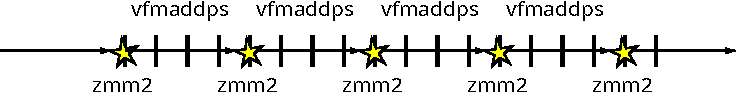
\includegraphics[width=0.6\textwidth]{out/pdf/svg/latency_1.pdf}
\end{center}

\end{frame}

%%%%%%%%%%%%%%%%%%%%%%%%%%%%%%%%%% 
\begin{frame}[fragile]
  \frametitle{CPU clocks vs. reference clocks}
  \begin{itemize}
  \item CPU changes clock frequency depending on the load (DVFS)
  \item reference clock runs at the same frequency (it is
    always proportional to the absolute time)
  \item an instruction takes a specified number of
    {\it CPU clocks}, not reference clocks
  \item the CPU clock is more predictable and thus
    more convenient for a precise reasoning of the code
  \end{itemize}

  \begin{center}
\begin{center}
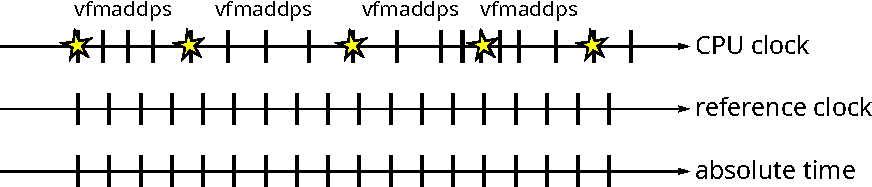
\includegraphics[width=0.8\textwidth]{out/pdf/svg/latency_2.pdf}
\end{center}
  \end{center}
\end{frame}

%%%%%%%%%%%%%%%%%%%%%%%%%%%%%%%%%% 
\section{Overcoming latency}
%%%%%%%%%%%%%%%%%%%%%%%%%%%%%%%%%% 
%%%%%%%%%%%%%%%%%%%%%%%%%%%%%%%%%% 
\begin{frame}[fragile]
\frametitle{How to overcome latencies?}

\begin{itemize}
\item increase parallelism (no other ways)!

\item<2-> you \ao{\em can't} make a serial chain of dependent computation
  run faster than determined by latencies

\begin{center}
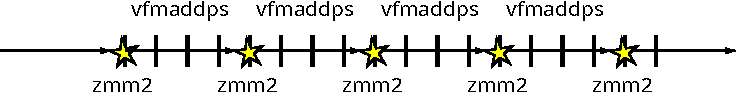
\includegraphics[width=0.6\textwidth]{out/pdf/svg/latency_1.pdf}
\end{center}

\item<3-> you \ao{\em can} only increase \ao{\em throughput},
  by running multiple {\it independent} chains

\begin{center}
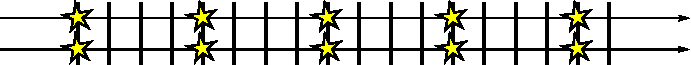
\includegraphics[width=0.6\textwidth]{out/pdf/svg/latency_3.pdf}
\end{center}

\item<4-> we expect the following to finish in 
  the same number of cycles as the original one,
  despite it performs twice as many flops

\begin{lstlisting}
for (i = 0; i < n; i++) {
  @\ao{\tt x0 = a * x0 + c}@;
  @\aka{\tt x1 = a * x1 + c}@;
}
\end{lstlisting}
\end{itemize}
\end{frame}

%%%%%%%%%%%%%%%%%%%%%%%%%%%%%%%%%% 
\begin{frame}[fragile]
\frametitle{Increase the number of chains further \ldots}
\begin{itemize}
\item we expect to reach peak FLOPS with $\geq 2 / (1/4) = 8$ chains
  (i.e., {\tt nv} $\geq 8$)
\begin{lstlisting}
long axpy_simd_c( ... ) {
  for (long i = 0; i < n; i++) {
    for (long j = 0; j < nv; j++) {
      X[j] = a * X[j] + c;
    } } }
\end{lstlisting}

\begin{center}
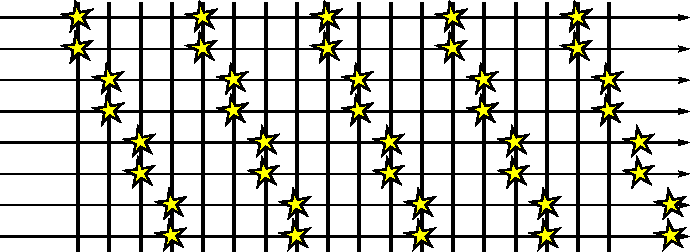
\includegraphics[width=0.6\textwidth]{out/pdf/svg/latency_4.pdf}
\end{center}

\item note: the above reasoning assumes a compiler's smartness
\item in particular, 
  {\tt X[j] = a * X[j] + c} is compiled into an FMA instruction
  on registers without load/store instructions
  (i.e., each of {\tt X[0], \ldots, X[7]} gets assigned a register)
\end{itemize}
\end{frame}

%%%%%%%%%%%%%%%%%%%%%%%%%%%%%%%%%% 
\begin{frame}[fragile]
\frametitle{Results}
\begin{columns}
\begin{column}{0.55\textwidth}
\begin{center}
  % {\scriptsize \input{out/tex/data/06axpy/simd_c_performance}}
  {\scriptsize % GNUPLOT: LaTeX picture with Postscript
\begingroup
  \makeatletter
  \providecommand\color[2][]{%
    \GenericError{(gnuplot) \space\space\space\@spaces}{%
      Package color not loaded in conjunction with
      terminal option `colourtext'%
    }{See the gnuplot documentation for explanation.%
    }{Either use 'blacktext' in gnuplot or load the package
      color.sty in LaTeX.}%
    \renewcommand\color[2][]{}%
  }%
  \providecommand\includegraphics[2][]{%
    \GenericError{(gnuplot) \space\space\space\@spaces}{%
      Package graphicx or graphics not loaded%
    }{See the gnuplot documentation for explanation.%
    }{The gnuplot epslatex terminal needs graphicx.sty or graphics.sty.}%
    \renewcommand\includegraphics[2][]{}%
  }%
  \providecommand\rotatebox[2]{#2}%
  \@ifundefined{ifGPcolor}{%
    \newif\ifGPcolor
    \GPcolortrue
  }{}%
  \@ifundefined{ifGPblacktext}{%
    \newif\ifGPblacktext
    \GPblacktexttrue
  }{}%
  % define a \g@addto@macro without @ in the name:
  \let\gplgaddtomacro\g@addto@macro
  % define empty templates for all commands taking text:
  \gdef\gplbacktext{}%
  \gdef\gplfronttext{}%
  \makeatother
  \ifGPblacktext
    % no textcolor at all
    \def\colorrgb#1{}%
    \def\colorgray#1{}%
  \else
    % gray or color?
    \ifGPcolor
      \def\colorrgb#1{\color[rgb]{#1}}%
      \def\colorgray#1{\color[gray]{#1}}%
      \expandafter\def\csname LTw\endcsname{\color{white}}%
      \expandafter\def\csname LTb\endcsname{\color{black}}%
      \expandafter\def\csname LTa\endcsname{\color{black}}%
      \expandafter\def\csname LT0\endcsname{\color[rgb]{1,0,0}}%
      \expandafter\def\csname LT1\endcsname{\color[rgb]{0,1,0}}%
      \expandafter\def\csname LT2\endcsname{\color[rgb]{0,0,1}}%
      \expandafter\def\csname LT3\endcsname{\color[rgb]{1,0,1}}%
      \expandafter\def\csname LT4\endcsname{\color[rgb]{0,1,1}}%
      \expandafter\def\csname LT5\endcsname{\color[rgb]{1,1,0}}%
      \expandafter\def\csname LT6\endcsname{\color[rgb]{0,0,0}}%
      \expandafter\def\csname LT7\endcsname{\color[rgb]{1,0.3,0}}%
      \expandafter\def\csname LT8\endcsname{\color[rgb]{0.5,0.5,0.5}}%
    \else
      % gray
      \def\colorrgb#1{\color{black}}%
      \def\colorgray#1{\color[gray]{#1}}%
      \expandafter\def\csname LTw\endcsname{\color{white}}%
      \expandafter\def\csname LTb\endcsname{\color{black}}%
      \expandafter\def\csname LTa\endcsname{\color{black}}%
      \expandafter\def\csname LT0\endcsname{\color{black}}%
      \expandafter\def\csname LT1\endcsname{\color{black}}%
      \expandafter\def\csname LT2\endcsname{\color{black}}%
      \expandafter\def\csname LT3\endcsname{\color{black}}%
      \expandafter\def\csname LT4\endcsname{\color{black}}%
      \expandafter\def\csname LT5\endcsname{\color{black}}%
      \expandafter\def\csname LT6\endcsname{\color{black}}%
      \expandafter\def\csname LT7\endcsname{\color{black}}%
      \expandafter\def\csname LT8\endcsname{\color{black}}%
    \fi
  \fi
    \setlength{\unitlength}{0.0500bp}%
    \ifx\gptboxheight\undefined%
      \newlength{\gptboxheight}%
      \newlength{\gptboxwidth}%
      \newsavebox{\gptboxtext}%
    \fi%
    \setlength{\fboxrule}{0.5pt}%
    \setlength{\fboxsep}{1pt}%
    \definecolor{tbcol}{rgb}{1,1,1}%
\begin{picture}(3400.00,2266.00)%
    \gplgaddtomacro\gplbacktext{%
      \csname LTb\endcsname%%
      \put(300,384){\makebox(0,0)[r]{\strut{}$0$}}%
      \put(300,574){\makebox(0,0)[r]{\strut{}$1$}}%
      \put(300,764){\makebox(0,0)[r]{\strut{}$2$}}%
      \put(300,954){\makebox(0,0)[r]{\strut{}$3$}}%
      \put(300,1145){\makebox(0,0)[r]{\strut{}$4$}}%
      \put(300,1335){\makebox(0,0)[r]{\strut{}$5$}}%
      \put(300,1525){\makebox(0,0)[r]{\strut{}$6$}}%
      \put(300,1715){\makebox(0,0)[r]{\strut{}$7$}}%
      \put(300,1905){\makebox(0,0)[r]{\strut{}$8$}}%
      \put(372,264){\makebox(0,0){\strut{}$0$}}%
      \put(672,264){\makebox(0,0){\strut{}$2$}}%
      \put(973,264){\makebox(0,0){\strut{}$4$}}%
      \put(1273,264){\makebox(0,0){\strut{}$6$}}%
      \put(1574,264){\makebox(0,0){\strut{}$8$}}%
      \put(1874,264){\makebox(0,0){\strut{}$10$}}%
      \put(2174,264){\makebox(0,0){\strut{}$12$}}%
      \put(2475,264){\makebox(0,0){\strut{}$14$}}%
      \put(2775,264){\makebox(0,0){\strut{}$16$}}%
      \put(2847,384){\makebox(0,0)[l]{\strut{}$0$}}%
      \put(2847,574){\makebox(0,0)[l]{\strut{}$8$}}%
      \put(2847,764){\makebox(0,0)[l]{\strut{}$16$}}%
      \put(2847,954){\makebox(0,0)[l]{\strut{}$24$}}%
      \put(2847,1145){\makebox(0,0)[l]{\strut{}$32$}}%
      \put(2847,1335){\makebox(0,0)[l]{\strut{}$40$}}%
      \put(2847,1525){\makebox(0,0)[l]{\strut{}$48$}}%
      \put(2847,1715){\makebox(0,0)[l]{\strut{}$56$}}%
      \put(2847,1905){\makebox(0,0)[l]{\strut{}$64$}}%
    }%
    \gplgaddtomacro\gplfronttext{%
      \csname LTb\endcsname%%
      \put(2208,1782){\makebox(0,0)[r]{\strut{}latency}}%
      \csname LTb\endcsname%%
      \put(2208,1662){\makebox(0,0)[r]{\strut{}throughput}}%
      \csname LTb\endcsname%%
      \put(114,1144){\rotatebox{-270.00}{\makebox(0,0){\strut{}cycles/iter}}}%
      \put(3123,1144){\rotatebox{-270.00}{\makebox(0,0){\strut{}flops/cycle}}}%
      \put(1573,84){\makebox(0,0){\strut{}variables}}%
      \put(1573,2085){\makebox(0,0){\strut{}a compile-time constant number of variables}}%
    }%
    \gplbacktext
    \put(0,0){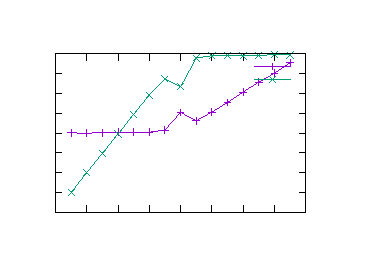
\includegraphics[width={170.00bp},height={113.30bp}]{out/tex/data/06axpb//cpu_latency_throughput_simd_c_big}}%
    \gplfronttext
  \end{picture}%
\endgroup
}
  % out/tex/data/06axpy/simd\_c\_performance
\end{center}

\begin{itemize}
\item []
\begin{lstlisting}
for (i = 0; i < n; i++) {
  @\ao{\tt x0 = a * x0 + b}@;
  @\aka{\tt x1 = a * x1 + b}@;
    ...
}
\end{lstlisting}
\end{itemize}
\end{column}
\begin{column}{0.01\textwidth}
\end{column}
\begin{column}{0.44\textwidth}
{\scriptsize
\begin{tabular}{|c|c|c|}\hline
chains & clocks/iter & flops/clock \\ \hline
1 & \mura{4.010} & 7.979 \\
2 & \mura{4.003} & 15.987 \\
3 & \mura{4.013} & 23.916 \\
4 & \mura{4.043} & 31.653 \\
5 & \mura{4.043} & 39.568 \\
6 & \mura{4.047} & 47.439 \\
7 & \mura{4.157} & 53.878 \\
8 & 5.044 & 50.751 \\
9 & 4.621 & 62.314 \\
10 & 5.057 & \ao{63.270} \\
11 & 5.549 & \ao{63.427} \\
12 & 6.076 & \ao{63.194} \\
13 & 6.573 & \ao{63.283} \\
14 & 7.022 & \ao{63.794} \\
15 & 7.552 & \ao{63.558} \\
\hline
\end{tabular}}
\end{column}    
\end{columns}

\end{frame}


%%%%%%%%%%%%%%%%%%%%%%%%%%%%%%%%%% 
%%%%%%%%%%%%%%%%%%%%%%%%%%%%%%%%%% 
\section{Superscalar processors}
%%%%%%%%%%%%%%%%%%%%%%%%%%%%%%%%%% 
%%%%%%%%%%%%%%%%%%%%%%%%%%%%%%%%%%

%%%%%%%%%%%%%%%%%%%%%%%%%%%%%%%%%% 
\begin{frame}
  \frametitle{Superscalar processors}
  how modern aggressive superscalar processors work:
\begin{itemize}
\item<2-> instruction decoding goes much ahead of actual executions
\item<3-> the actual execution of an instruction
  does not happen until, and happens as soon as,
  \ao{\emph{its operands and execution resources are ready}}
  \emph{(out of order execution)}
\item<4-> $\Rightarrow$ as a crude approximation,
  performance is constrained by 
  \begin{itemize}
  \item<5-> \ao{\emph{latency:}} imposed by {\it dependencies}
    between instructions
  \item<6-> \ao{\emph{throughput:}}
    imposed by execution resources of the processor
    (e.g., two fmadds/cycle)
  \end{itemize}
\end{itemize}
\end{frame}

%%%%%%%%%%%%%%%%%%%%%%%%%%%%%%%%%% 
\begin{frame}
  \frametitle{A general theory of workload performance on aggressive superscalar machines}
  \begin{itemize}
  \item \ao{\it dependency} constrains how fast a computation can proceed,
    even if there are infinite number of execution resources
    
  \item increase the number of independent computations and
    you increase \ao{\it throughput}, until it hits the limit
    of execution resources

\begin{center}
% {\scriptsize \input{out/tex/data/06axpy/simd_c_performance}}
  {\scriptsize % GNUPLOT: LaTeX picture with Postscript
\begingroup
  \makeatletter
  \providecommand\color[2][]{%
    \GenericError{(gnuplot) \space\space\space\@spaces}{%
      Package color not loaded in conjunction with
      terminal option `colourtext'%
    }{See the gnuplot documentation for explanation.%
    }{Either use 'blacktext' in gnuplot or load the package
      color.sty in LaTeX.}%
    \renewcommand\color[2][]{}%
  }%
  \providecommand\includegraphics[2][]{%
    \GenericError{(gnuplot) \space\space\space\@spaces}{%
      Package graphicx or graphics not loaded%
    }{See the gnuplot documentation for explanation.%
    }{The gnuplot epslatex terminal needs graphicx.sty or graphics.sty.}%
    \renewcommand\includegraphics[2][]{}%
  }%
  \providecommand\rotatebox[2]{#2}%
  \@ifundefined{ifGPcolor}{%
    \newif\ifGPcolor
    \GPcolortrue
  }{}%
  \@ifundefined{ifGPblacktext}{%
    \newif\ifGPblacktext
    \GPblacktexttrue
  }{}%
  % define a \g@addto@macro without @ in the name:
  \let\gplgaddtomacro\g@addto@macro
  % define empty templates for all commands taking text:
  \gdef\gplbacktext{}%
  \gdef\gplfronttext{}%
  \makeatother
  \ifGPblacktext
    % no textcolor at all
    \def\colorrgb#1{}%
    \def\colorgray#1{}%
  \else
    % gray or color?
    \ifGPcolor
      \def\colorrgb#1{\color[rgb]{#1}}%
      \def\colorgray#1{\color[gray]{#1}}%
      \expandafter\def\csname LTw\endcsname{\color{white}}%
      \expandafter\def\csname LTb\endcsname{\color{black}}%
      \expandafter\def\csname LTa\endcsname{\color{black}}%
      \expandafter\def\csname LT0\endcsname{\color[rgb]{1,0,0}}%
      \expandafter\def\csname LT1\endcsname{\color[rgb]{0,1,0}}%
      \expandafter\def\csname LT2\endcsname{\color[rgb]{0,0,1}}%
      \expandafter\def\csname LT3\endcsname{\color[rgb]{1,0,1}}%
      \expandafter\def\csname LT4\endcsname{\color[rgb]{0,1,1}}%
      \expandafter\def\csname LT5\endcsname{\color[rgb]{1,1,0}}%
      \expandafter\def\csname LT6\endcsname{\color[rgb]{0,0,0}}%
      \expandafter\def\csname LT7\endcsname{\color[rgb]{1,0.3,0}}%
      \expandafter\def\csname LT8\endcsname{\color[rgb]{0.5,0.5,0.5}}%
    \else
      % gray
      \def\colorrgb#1{\color{black}}%
      \def\colorgray#1{\color[gray]{#1}}%
      \expandafter\def\csname LTw\endcsname{\color{white}}%
      \expandafter\def\csname LTb\endcsname{\color{black}}%
      \expandafter\def\csname LTa\endcsname{\color{black}}%
      \expandafter\def\csname LT0\endcsname{\color{black}}%
      \expandafter\def\csname LT1\endcsname{\color{black}}%
      \expandafter\def\csname LT2\endcsname{\color{black}}%
      \expandafter\def\csname LT3\endcsname{\color{black}}%
      \expandafter\def\csname LT4\endcsname{\color{black}}%
      \expandafter\def\csname LT5\endcsname{\color{black}}%
      \expandafter\def\csname LT6\endcsname{\color{black}}%
      \expandafter\def\csname LT7\endcsname{\color{black}}%
      \expandafter\def\csname LT8\endcsname{\color{black}}%
    \fi
  \fi
    \setlength{\unitlength}{0.0500bp}%
    \ifx\gptboxheight\undefined%
      \newlength{\gptboxheight}%
      \newlength{\gptboxwidth}%
      \newsavebox{\gptboxtext}%
    \fi%
    \setlength{\fboxrule}{0.5pt}%
    \setlength{\fboxsep}{1pt}%
    \definecolor{tbcol}{rgb}{1,1,1}%
\begin{picture}(3400.00,2266.00)%
    \gplgaddtomacro\gplbacktext{%
      \csname LTb\endcsname%%
      \put(300,384){\makebox(0,0)[r]{\strut{}$0$}}%
      \put(300,574){\makebox(0,0)[r]{\strut{}$1$}}%
      \put(300,764){\makebox(0,0)[r]{\strut{}$2$}}%
      \put(300,954){\makebox(0,0)[r]{\strut{}$3$}}%
      \put(300,1145){\makebox(0,0)[r]{\strut{}$4$}}%
      \put(300,1335){\makebox(0,0)[r]{\strut{}$5$}}%
      \put(300,1525){\makebox(0,0)[r]{\strut{}$6$}}%
      \put(300,1715){\makebox(0,0)[r]{\strut{}$7$}}%
      \put(300,1905){\makebox(0,0)[r]{\strut{}$8$}}%
      \put(372,264){\makebox(0,0){\strut{}$0$}}%
      \put(672,264){\makebox(0,0){\strut{}$2$}}%
      \put(973,264){\makebox(0,0){\strut{}$4$}}%
      \put(1273,264){\makebox(0,0){\strut{}$6$}}%
      \put(1574,264){\makebox(0,0){\strut{}$8$}}%
      \put(1874,264){\makebox(0,0){\strut{}$10$}}%
      \put(2174,264){\makebox(0,0){\strut{}$12$}}%
      \put(2475,264){\makebox(0,0){\strut{}$14$}}%
      \put(2775,264){\makebox(0,0){\strut{}$16$}}%
      \put(2847,384){\makebox(0,0)[l]{\strut{}$0$}}%
      \put(2847,574){\makebox(0,0)[l]{\strut{}$8$}}%
      \put(2847,764){\makebox(0,0)[l]{\strut{}$16$}}%
      \put(2847,954){\makebox(0,0)[l]{\strut{}$24$}}%
      \put(2847,1145){\makebox(0,0)[l]{\strut{}$32$}}%
      \put(2847,1335){\makebox(0,0)[l]{\strut{}$40$}}%
      \put(2847,1525){\makebox(0,0)[l]{\strut{}$48$}}%
      \put(2847,1715){\makebox(0,0)[l]{\strut{}$56$}}%
      \put(2847,1905){\makebox(0,0)[l]{\strut{}$64$}}%
    }%
    \gplgaddtomacro\gplfronttext{%
      \csname LTb\endcsname%%
      \put(2208,1782){\makebox(0,0)[r]{\strut{}latency}}%
      \csname LTb\endcsname%%
      \put(2208,1662){\makebox(0,0)[r]{\strut{}throughput}}%
      \csname LTb\endcsname%%
      \put(114,1144){\rotatebox{-270.00}{\makebox(0,0){\strut{}cycles/iter}}}%
      \put(3123,1144){\rotatebox{-270.00}{\makebox(0,0){\strut{}flops/cycle}}}%
      \put(1573,84){\makebox(0,0){\strut{}variables}}%
      \put(1573,2085){\makebox(0,0){\strut{}a compile-time constant number of variables}}%
    }%
    \gplbacktext
    \put(0,0){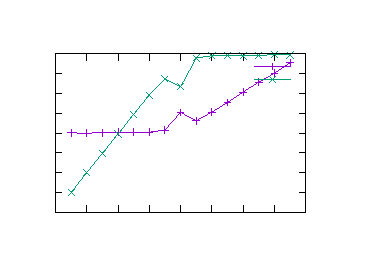
\includegraphics[width={170.00bp},height={113.30bp}]{out/tex/data/06axpb//cpu_latency_throughput_simd_c_big}}%
    \gplfronttext
  \end{picture}%
\endgroup
}
%  out/tex/data/06axpy/simd\_c\_performance
\end{center}
  \end{itemize}
\end{frame}



%%%%%%%%%%%%%%%%%%%%%%%%%%%%%%%%%% 
\begin{frame}
\frametitle{A more general understanding about \ao{\em throughput} limits}

\begin{itemize}
\item \ao{\emph{what you need to know:}}
  \begin{quote}
    all instructions have their own throughput limits (just like FMA),
    due to execution resources
  \end{quote}

\item some examples of recent Intel CPUs

  \begin{center}
{\scriptsize
  \begin{tabular}{|l|c|c|c|}\hline
instruction           & Broadwell & Skylake SP & Ice Lake SP \\\hline
  fp add/mul/fmadd    & 2         & 2         & 2 \\
  load                & 2         & 2         & 2 \\
  store               & 1         & 1         & \ao{2} \\
  typical integer ops & 4         & 4         & 4  \\
  \ldots              & \ldots    & \ldots    & \ldots \\
\hline
  \end{tabular}
}
\end{center}

\item e.g., a loop containing 10 load instructions takes 
  $\geq 10/2 = 5$ cycless/iteration

\item different but similar instructions may use the same execution resource
  so may be subject of the same limitation
\item a more general reasoning $\Rightarrow$ \ao{\it dispatch ports}
\end{itemize}

% \begin{columns}
% \begin{column}{0.6\textwidth}
% \begin{center}
% 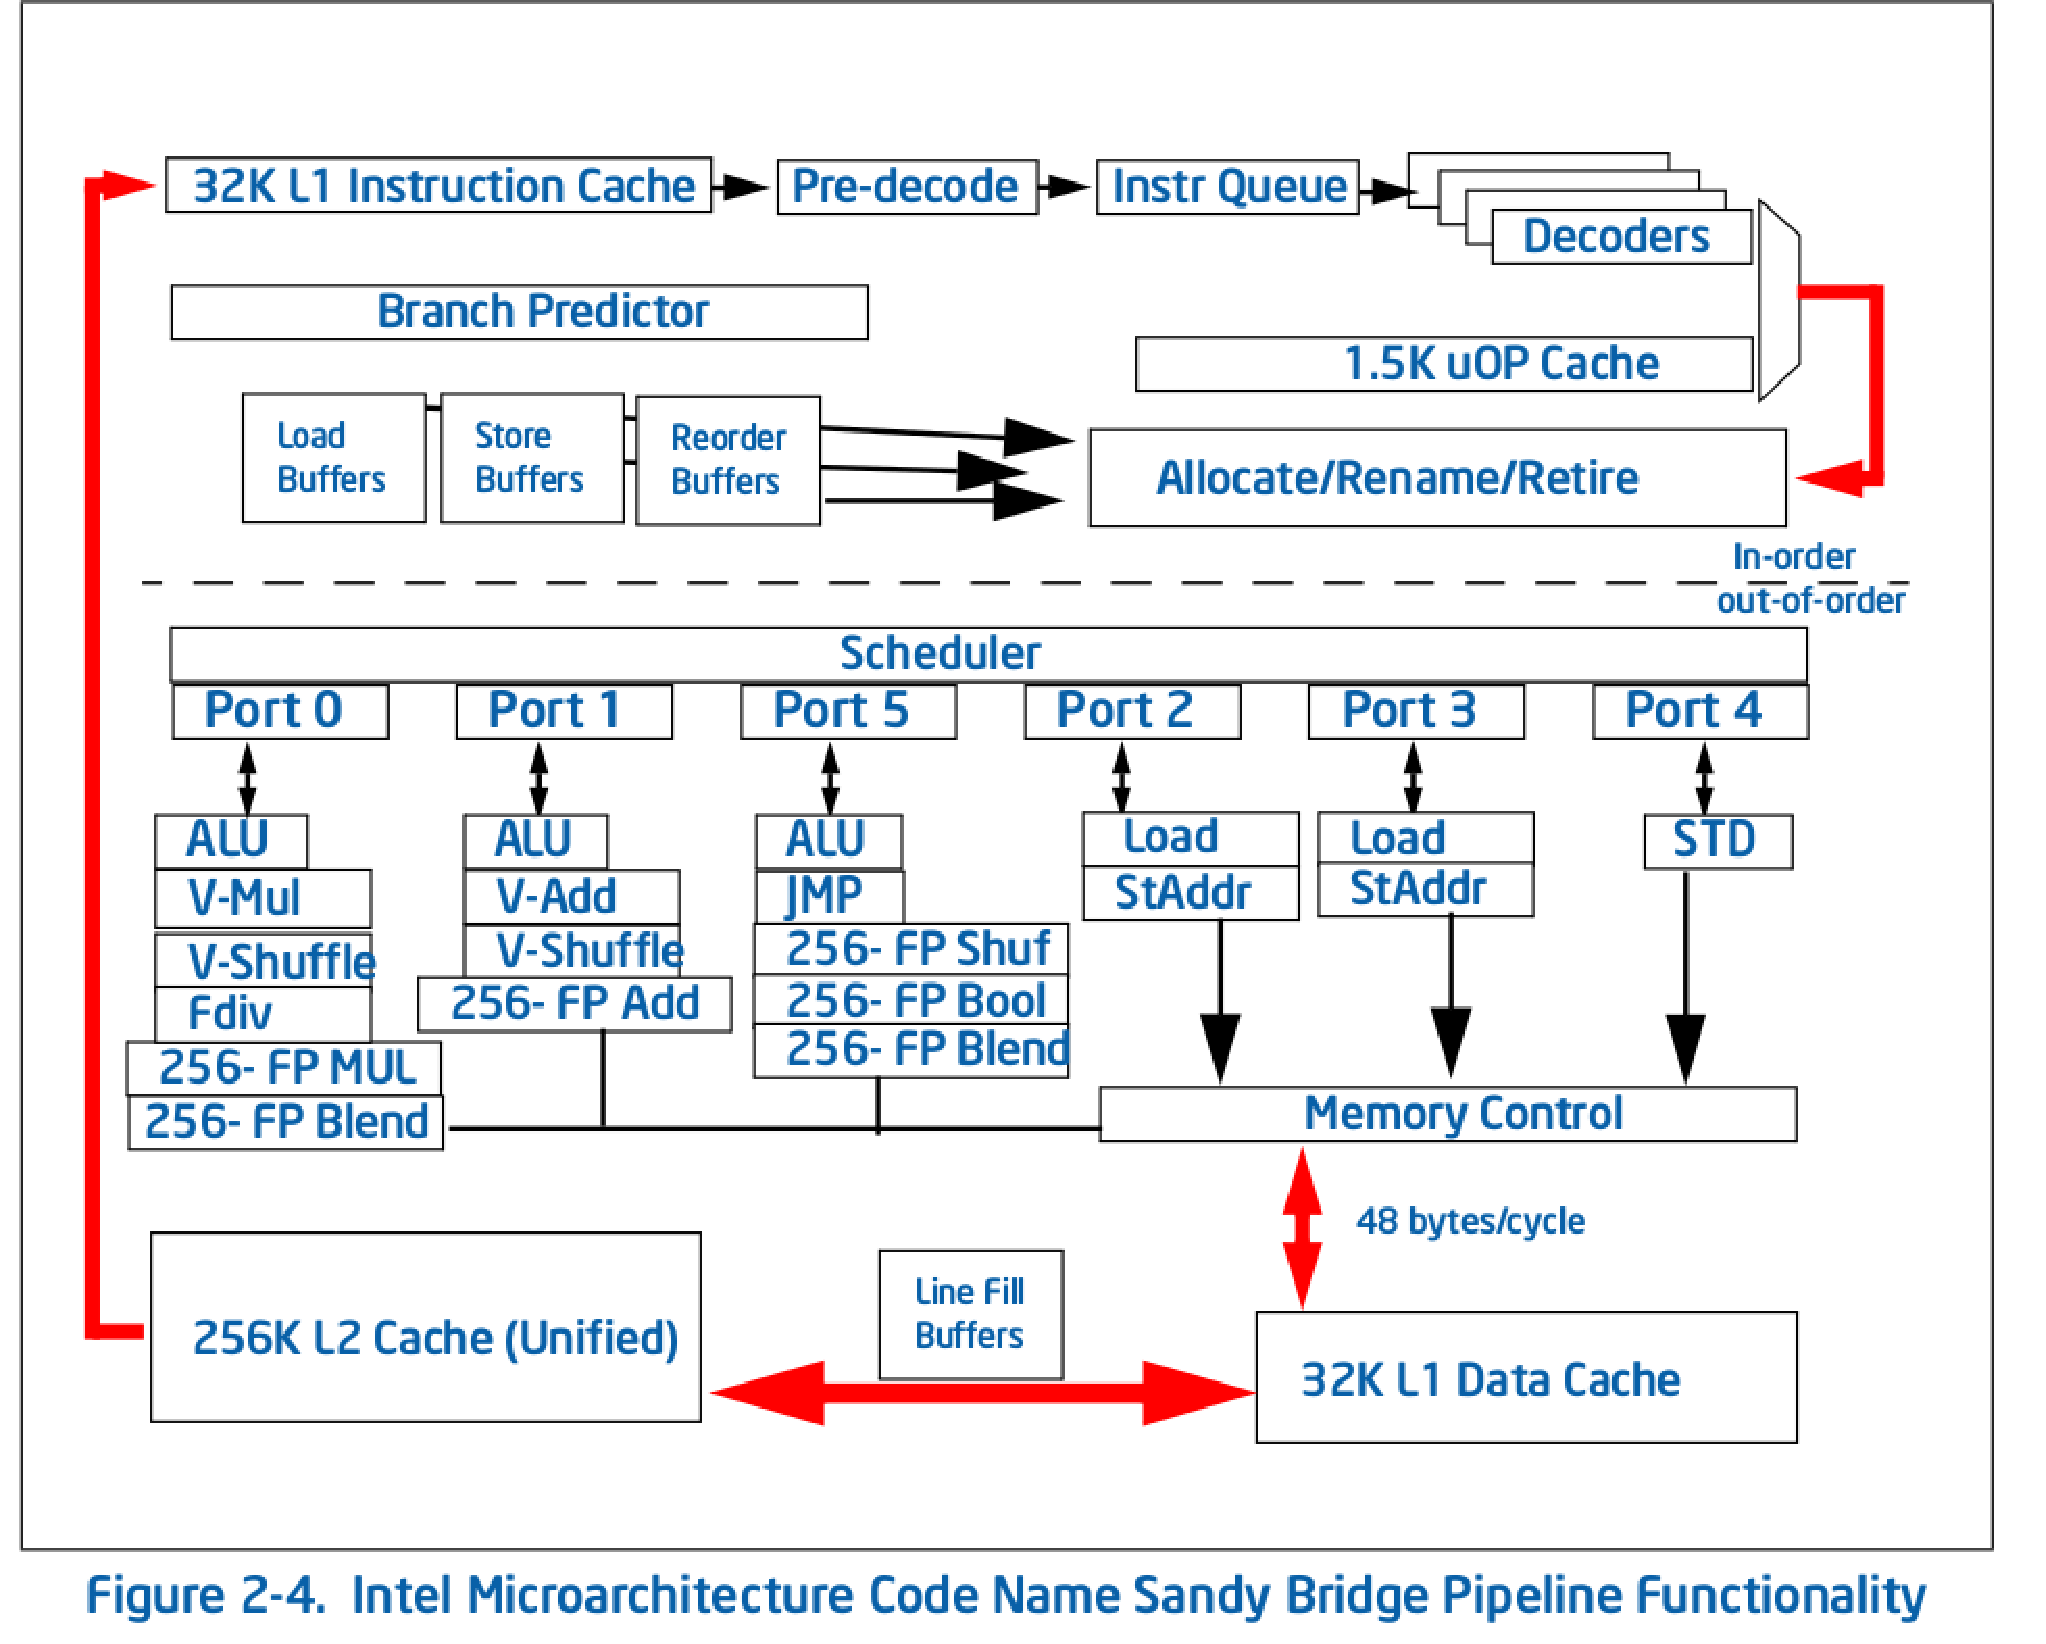
\includegraphics[width=0.8\textwidth]{out/pdf/img/sandybridge.pdf}

% {\tiny\em Intel 64 and IA-32 Architecture Optimization Reference Manual}
% \end{center}
% \end{column}
% \end{columns}
\end{frame}


%%%%%%%%%%%%%%%%%%%%%%%%%%%%%%%%%%
\iffalse
\begin{frame}
\frametitle{Some representative throughput limits}

\begin{itemize}
\item throughput of a particular instruction $=$ the maximum number of
  {\it that} instruction that can be executed in a cycle

\begin{center}
{\small
  \begin{tabular}{|l|c|c|c|}\hline
instruction           & Broadwell & Skylake SP & Ice Lake SP \\\hline
  fp add/mul/fmadd    & 2         & 2         & 2 \\
  load                & 2         & 2         & 2 \\
  store               & 1         & 1         & \ao{2} \\
  typical integer ops & 4         & 4         & 4  \\
  \ldots              & \ldots    & \ldots    & \ldots \\
\hline
  \end{tabular}
}
\end{center}

e.g.,

  \begin{itemize}
  \item you can't execute a loop containing 10 load instructions
    faster than $10/2 = 5$ clocks/iteration
  \item you can't execute a loop containing 7 store instructions
    faster than $7$ clocks/iteration on Skylake SP and earlier
  \end{itemize}
  
\item not surprisingly, different but similar instructions may
  share execution resources so may be subject of the same limitation
\item a more general reasoning $\Rightarrow$ {\it dispatch ports}
\end{itemize}
\end{frame}
\fi

%%%%%%%%%%%%%%%%%%%%%%%%%%%%%%%%%% 
\begin{frame}[fragile]
\frametitle{Dispatch ports}
\begin{columns}
\begin{column}{0.47\textwidth}
\begin{itemize}
\item each instruction ($\mu$-operation) 
  is dispatched to a specific execution unit through a \ao{\emph{dispatch port}}
\item each port can take only a single operation per cycle
\item this determines the throughput of all instructions
  that go to that port
\item \ao{\it with destination ports of instructions, one can calculate
    the throughput limit of a given loop}
\end{itemize}
\end{column}
% https://cdrdv2-public.intel.com/671488/248966_software_optimization_manual.pdf

\begin{column}{0.56\textwidth}
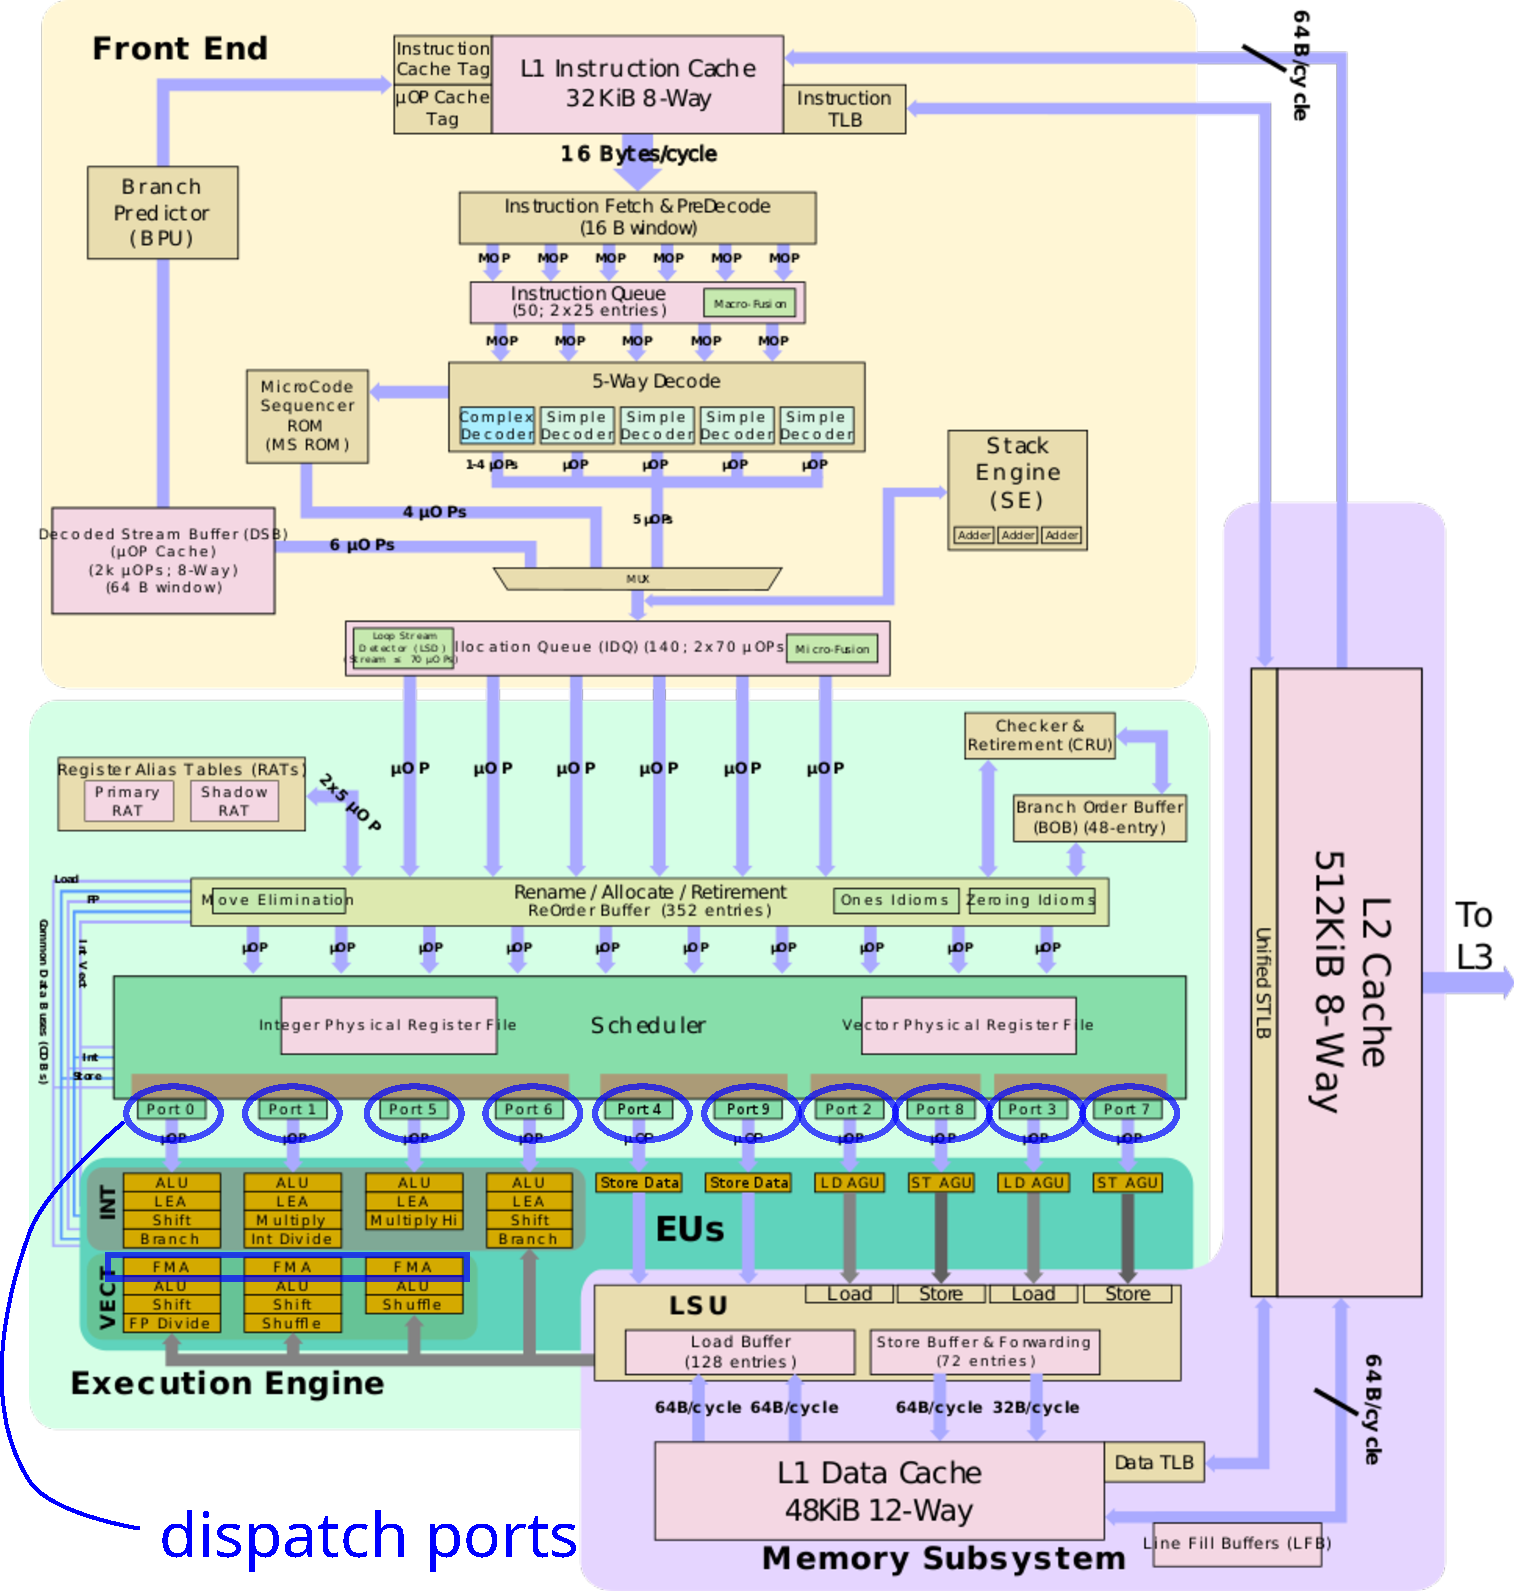
\includegraphics[width=\textwidth]{out/pdf/svg/icelake.pdf}

{\tiny Chipwikia - \href{https://en.wikipedia.org/wiki/Sunny_Cove_(microarchitecture)}{Sunny cove architecture}, CC BY-SA 4.0, \url{https://commons.wikimedia.org/w/index.php?curid=122557706}}

\end{column}
\end{columns}
\end{frame}


%%%%%%%%%%%%%%%%%%%%%%%%%%%%%%%%%%
\iffalse
\begin{frame}[fragile]
\frametitle{Dispatch ports}
\begin{columns}
\begin{column}{0.5\textwidth}
\begin{itemize}
\item each instruction ($\mu$-operation) 
  is dispatched to a specific \ao{\emph{port}}
\item Skylake X ports
  \begin{itemize}
  \item fmadd $\rightarrow$ port 0 or 1
  \item load $\rightarrow$ port 2 or 3
  \item store $\rightarrow$ port 4
  \item load/store address generation $\rightarrow$ port 7
  \item int $\rightarrow$ port 0, 1, 5, or 6
  \item etc.
  \end{itemize}

\end{itemize}
\end{column}

\begin{column}{0.5\textwidth}
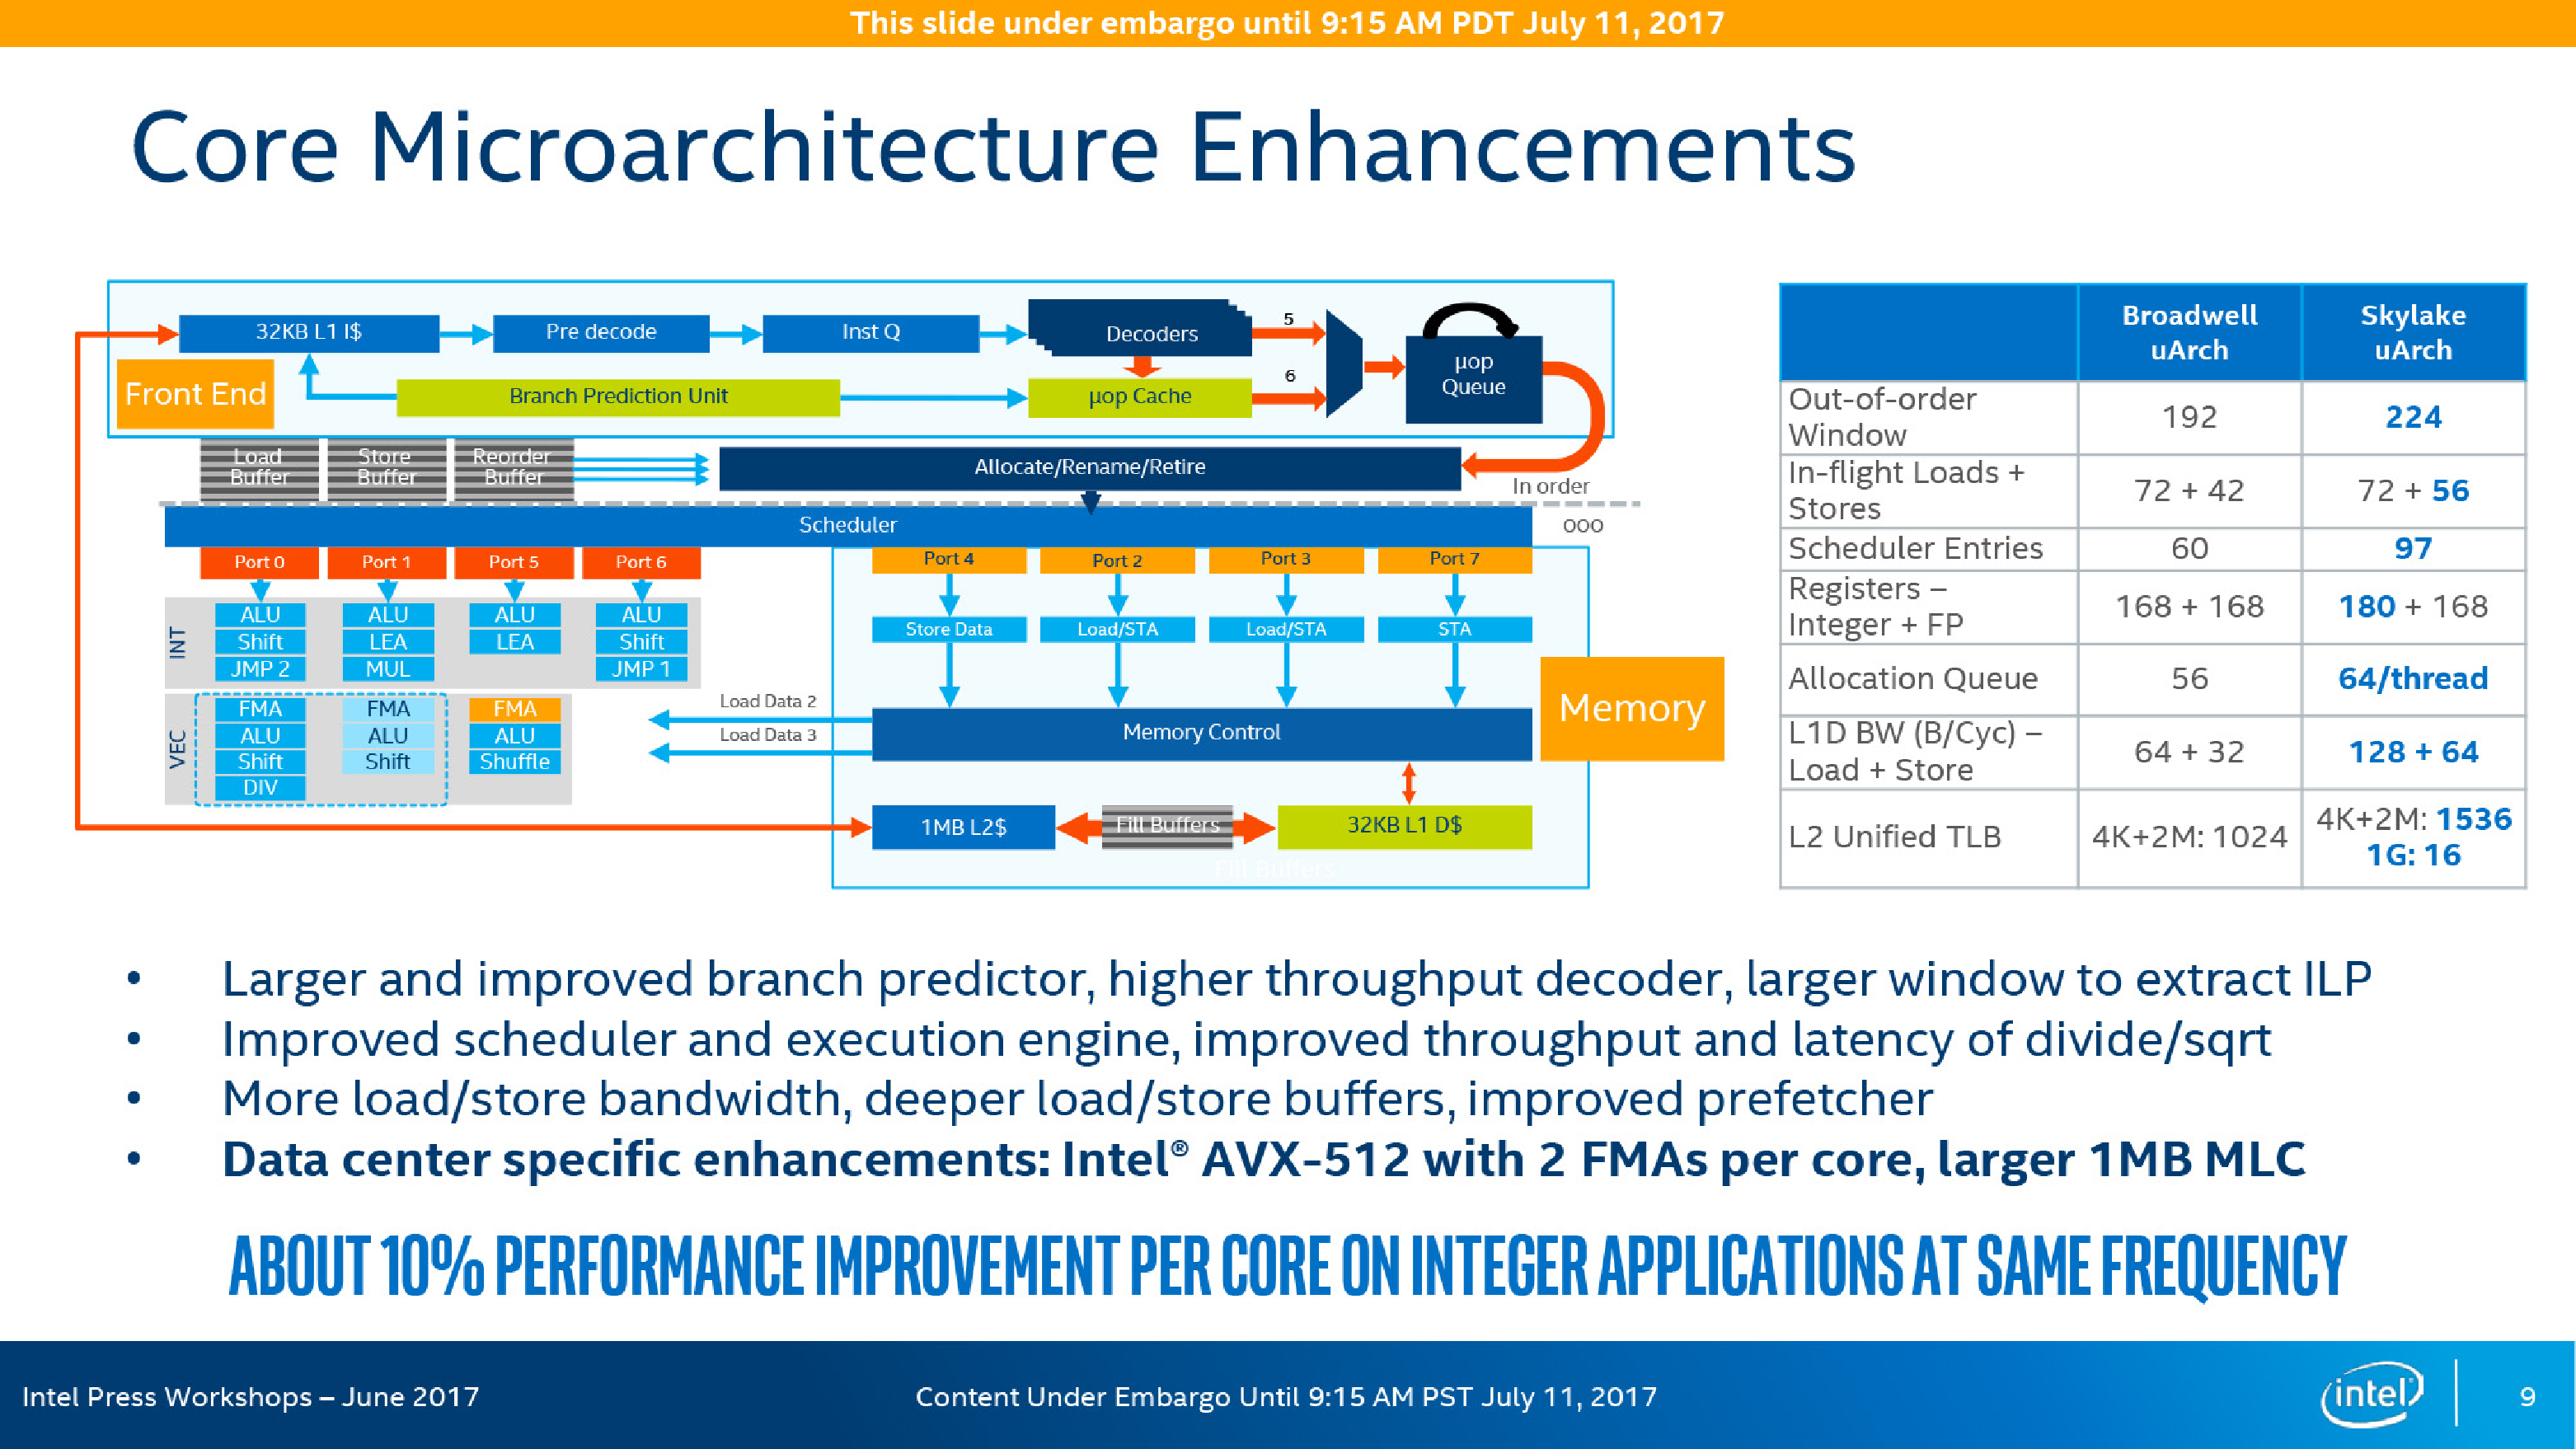
\includegraphics[width=\textwidth]{out/pdf/img/skylake_sp_buffer_windows.pdf}
{\tiny source: \url{https://en.wikichip.org/wiki/intel/microarchitectures/skylake_(server)}}
\end{column}
\end{columns}

\begin{itemize}
\item each port can take only a single operation per cycle
  \begin{itemize}
  \item this determines the aggregate throughput of all instructions
    that go to that port
  \end{itemize}
\item \ao{\it with destination ports of instructions, one can calculate
    the throughput limit of a given loop}
\end{itemize}
\end{frame}
\fi

%%%%%%%%%%%%%%%%%%%%%%%%%%%%%%%%%%
\begin{frame}[fragile]
\frametitle{LLVM Machine Code Analyzer ({\tt llvm-mca})}

\begin{itemize}
\item a great tool to analyze
  the throughput (and latency to some extent) limit

\item given a code sequence, it shows
  \begin{itemize}
  \item \ao{latency} and
  \item \ao{dispatch port}
  \end{itemize}
  of each instruction and, based on them \ao{calculates
  the number of cycles per iteration},
\item under some simplifying assumptions
  \begin{itemize}
  \item the given sequence repeats many times
  \item no cache misses (!)
  \item no dependencies through memory (load does not depend on earlier stores)
  \item no branch misprediction
  \end{itemize}

\item $\Rightarrow$ a great tool to analyze the innermost, straight sequence of
  instructions without branches (basic blocks)
\end{itemize}
\end{frame}

%%%%%%%%%%%%%%%%%%%%%%%%%%%%%%%%%%
\begin{frame}[fragile]
\frametitle{How to use {\tt llvm-mca}}
\begin{enumerate}
\item generate assembly (get {\tt program.s}) by, e.g.,
\begin{lstlisting}
clang -O3 -mavx512f -mfma ... program.c @{\ao{\tt -S}}@
\end{lstlisting}      
\item find the loop 
  you want to analyze in the assembly

\item sandwich it by \ao{\tt \# LLVM-MCA-BEGIN} and \ao{\tt \# LLVM-MCA-END}
\begin{lstlisting}
@\ao{\tt \# LLVM-MCA-BEGIN}@
.L123
   ...
   ...
   jne .L123
@\ao{\tt \# LLVM-MCA-END}@
\end{lstlisting}
\item run {\tt llvm-mca} tool on the assembly code
\begin{lstlisting}
llvm-mca program.s    
\end{lstlisting}
\end{enumerate}
\end{frame}

%%%%%%%%%%%%%%%%%%%%%%%%%%%%%%%%%%
\begin{frame}[fragile]
  \frametitle{How to use {\tt llvm-mca}}
  \begin{itemize}
  \item it shows 
    \begin{itemize}
    \item latency of each instruction
    \item dispatch port used by each instruction
    \end{itemize}
    and how many instructions use each of the dispatch ports
    (therefore the throughput limit of the loop)
  \item with {\tt --timeline} option, 
\begin{lstlisting}
llvm-mca --timeline program.s    
\end{lstlisting}
it also shows when each instruction gets decoded, dispatched, and finished
(particularly instructive)
\end{itemize}
\end{frame}


%%%%%%%%%%%%%%%%%%%%%%%%%%%%%%%%%%
\begin{frame}[fragile]
  \frametitle{Example}
  \begin{itemize}
  \item input (assembly)
{\tiny\begin{lstlisting}
@\ao{\tt \# LLVM-MCA-BEGIN}@
.LBB3_8:
 # xmm0 = (xmm1 * xmm0) + xmm2
 vfmadd213sd %xmm2, %xmm1, %xmm0
 vfmadd213sd %xmm2, %xmm1, %xmm0
 vfmadd213sd %xmm2, %xmm1, %xmm0
 vfmadd213sd %xmm2, %xmm1, %xmm0
 vfmadd213sd %xmm2, %xmm1, %xmm0
 vfmadd213sd %xmm2, %xmm1, %xmm0
 vfmadd213sd %xmm2, %xmm1, %xmm0
 vfmadd213sd %xmm2, %xmm1, %xmm0
 addq $-8, %rax
 jne .LBB3_8
@\ao{\tt \# LLVM-MCA-END}@
\end{lstlisting} %$
}
\end{itemize}
\end{frame}

%%%%%%%%%%%%%%%%%%%%%%%%%%%%%%%%%%
\begin{frame}[fragile]
  \frametitle{Example}
  \begin{itemize}
\item output (dispatch port used by each instruction)
{\tiny\begin{lstlisting}
Resource pressure by instruction:
[0]  [1]  [2]  [3]  [4] .. [11] Instructions:
 -    -   0.99 0.01  -      -   vfmadd213sd %xmm2, %xmm1, %xmm0
 -    -    -   1.00  -      -   vfmadd213sd %xmm2, %xmm1, %xmm0
 -    -   0.99 0.01  -      -   vfmadd213sd %xmm2, %xmm1, %xmm0
 -    -    -   1.00  -      -   vfmadd213sd %xmm2, %xmm1, %xmm0
 -    -   1.00  -    -      -   vfmadd213sd %xmm2, %xmm1, %xmm0
 -    -    -   1.00  -      -   vfmadd213sd %xmm2, %xmm1, %xmm0
 -    -   1.00  -    -      -   vfmadd213sd %xmm2, %xmm1, %xmm0
 -    -    -   1.00  -      -   vfmadd213sd %xmm2, %xmm1, %xmm0
 -    -    -   0.01  -      -   addq $-8, %rax
 -    -   0.04  -    -      -   jne .LBB3_8
\end{lstlisting}%$
}
\end{itemize}
\end{frame}

%%%%%%%%%%%%%%%%%%%%%%%%%%%%%%%%%%
\begin{frame}[fragile]
  \frametitle{Example}
  \begin{itemize}
\item output (timeline)
{\tiny
\begin{lstlisting}
           ...
D=====...==eeee@\ao{\tt E}@R   .    .    .    .  vfmadd213sd %xmm2, %xmm1, %xmm0
.D====...======@\ao{\tt e}@eee@\aka{\tt E}@R    .    .    .  vfmadd213sd %xmm2, %xmm1, %xmm0
.D====...==========@\aka{\tt e}@eee@\ore{\tt E}@R.    .    .  vfmadd213sd %xmm2, %xmm1, %xmm0
.DeE--...---------------R.    .    .  addq $-8, %rax
.D=eE-...---------------R.    .    .  jne .LBB3_8
.D====...==============@\ore{\tt e}@eee@\mido{\tt E}@R .    .  vfmadd213sd %xmm2, %xmm1, %xmm0
.D====...==================@\mido{\tt e}@eeeER  .  vfmadd213sd %xmm2, %xmm1, %xmm0
. D===...======================eeeeER vfmadd213sd %xmm2, %xmm1, %xmm0
           ...
\end{lstlisting}%$
}
\end{itemize}
\end{frame}


%%%%%%%%%%%%%%%%%%%%%%%%%%%%%%%%%% 
%%%%%%%%%%%%%%%%%%%%%%%%%%%%%%%%%%
\iffalse
\section{A slightly more realistic example}
%%%%%%%%%%%%%%%%%%%%%%%%%%%%%%%%%% 
%%%%%%%%%%%%%%%%%%%%%%%%%%%%%%%%%%

%%%%%%%%%%%%%%%%%%%%%%%%%%%%%%%%%% 
\begin{frame}[fragile]
\frametitle{What if the number of chains is a variable?}
\begin{itemize}
\item purpose: illustrate the same concept with a slightly
  more complex/common case
  
\item let's try the following code, identical to the one we
  successfully achieved nearly peak performance for,
  except that \ao{\it the number of variables (m) is now a
  variable} (not a compile-time constant)
\begin{lstlisting}
void axpy_simd_m(..., @\ao{\texttt{long m}}@) { 
  for (long i = 0; i < n; i++) {
    for (long j = 0; j < m; j++) {
      X[j] = a * X[j] + c;
    } } }
\end{lstlisting}

\end{itemize}
\end{frame}


%%%%%%%%%%%%%%%%%%%%%%%%%%%%%%%%%% 
\begin{frame}
\frametitle{When we experiment \ldots}

\begin{columns}
\begin{column}{0.35\textwidth}
\begin{center}
{\scriptsize
\begin{tabular}{|c|c|c|}\hline
chains & clocks/iter & flops/clock \\
  \hline
1 & \mura{11.034} & 2.899 \\
2 & \mura{11.062} & 5.785 \\
3 & \mura{11.047} & 8.689 \\
4 & \mura{11.150} & 11.479 \\
5 & 11.199 & 14.286 \\
6 & 11.308 & 16.951 \\
7 & 11.389 & 19.666 \\
8 & 12.174 & 21.027 \\
9 & 13.159 & 21.885 \\
10 & 14.071 & 22.741 \\
$\cdots$ & $\cdots$ & $\cdots$ \\
17 & 22.977 & \ao{23.675} \\
18 & 24.171 & \ao{23.829} \\
19 & 25.345 & \ao{23.988} \\
20 & 26.605 & \ao{24.055} \\
\hline
\end{tabular}}
\end{center}
\end{column}

\begin{column}{0.65\textwidth}
\begin{center}
%{\scriptsize \input{out/tex/data/06axpy/simd_m_performance}}
  {\scriptsize % GNUPLOT: LaTeX picture with Postscript
\begingroup
  \makeatletter
  \providecommand\color[2][]{%
    \GenericError{(gnuplot) \space\space\space\@spaces}{%
      Package color not loaded in conjunction with
      terminal option `colourtext'%
    }{See the gnuplot documentation for explanation.%
    }{Either use 'blacktext' in gnuplot or load the package
      color.sty in LaTeX.}%
    \renewcommand\color[2][]{}%
  }%
  \providecommand\includegraphics[2][]{%
    \GenericError{(gnuplot) \space\space\space\@spaces}{%
      Package graphicx or graphics not loaded%
    }{See the gnuplot documentation for explanation.%
    }{The gnuplot epslatex terminal needs graphicx.sty or graphics.sty.}%
    \renewcommand\includegraphics[2][]{}%
  }%
  \providecommand\rotatebox[2]{#2}%
  \@ifundefined{ifGPcolor}{%
    \newif\ifGPcolor
    \GPcolortrue
  }{}%
  \@ifundefined{ifGPblacktext}{%
    \newif\ifGPblacktext
    \GPblacktexttrue
  }{}%
  % define a \g@addto@macro without @ in the name:
  \let\gplgaddtomacro\g@addto@macro
  % define empty templates for all commands taking text:
  \gdef\gplbacktext{}%
  \gdef\gplfronttext{}%
  \makeatother
  \ifGPblacktext
    % no textcolor at all
    \def\colorrgb#1{}%
    \def\colorgray#1{}%
  \else
    % gray or color?
    \ifGPcolor
      \def\colorrgb#1{\color[rgb]{#1}}%
      \def\colorgray#1{\color[gray]{#1}}%
      \expandafter\def\csname LTw\endcsname{\color{white}}%
      \expandafter\def\csname LTb\endcsname{\color{black}}%
      \expandafter\def\csname LTa\endcsname{\color{black}}%
      \expandafter\def\csname LT0\endcsname{\color[rgb]{1,0,0}}%
      \expandafter\def\csname LT1\endcsname{\color[rgb]{0,1,0}}%
      \expandafter\def\csname LT2\endcsname{\color[rgb]{0,0,1}}%
      \expandafter\def\csname LT3\endcsname{\color[rgb]{1,0,1}}%
      \expandafter\def\csname LT4\endcsname{\color[rgb]{0,1,1}}%
      \expandafter\def\csname LT5\endcsname{\color[rgb]{1,1,0}}%
      \expandafter\def\csname LT6\endcsname{\color[rgb]{0,0,0}}%
      \expandafter\def\csname LT7\endcsname{\color[rgb]{1,0.3,0}}%
      \expandafter\def\csname LT8\endcsname{\color[rgb]{0.5,0.5,0.5}}%
    \else
      % gray
      \def\colorrgb#1{\color{black}}%
      \def\colorgray#1{\color[gray]{#1}}%
      \expandafter\def\csname LTw\endcsname{\color{white}}%
      \expandafter\def\csname LTb\endcsname{\color{black}}%
      \expandafter\def\csname LTa\endcsname{\color{black}}%
      \expandafter\def\csname LT0\endcsname{\color{black}}%
      \expandafter\def\csname LT1\endcsname{\color{black}}%
      \expandafter\def\csname LT2\endcsname{\color{black}}%
      \expandafter\def\csname LT3\endcsname{\color{black}}%
      \expandafter\def\csname LT4\endcsname{\color{black}}%
      \expandafter\def\csname LT5\endcsname{\color{black}}%
      \expandafter\def\csname LT6\endcsname{\color{black}}%
      \expandafter\def\csname LT7\endcsname{\color{black}}%
      \expandafter\def\csname LT8\endcsname{\color{black}}%
    \fi
  \fi
    \setlength{\unitlength}{0.0500bp}%
    \ifx\gptboxheight\undefined%
      \newlength{\gptboxheight}%
      \newlength{\gptboxwidth}%
      \newsavebox{\gptboxtext}%
    \fi%
    \setlength{\fboxrule}{0.5pt}%
    \setlength{\fboxsep}{1pt}%
    \definecolor{tbcol}{rgb}{1,1,1}%
\begin{picture}(3400.00,2266.00)%
    \gplgaddtomacro\gplbacktext{%
      \csname LTb\endcsname%%
      \put(372,384){\makebox(0,0)[r]{\strut{}$0$}}%
      \put(372,638){\makebox(0,0)[r]{\strut{}$5$}}%
      \put(372,891){\makebox(0,0)[r]{\strut{}$10$}}%
      \put(372,1145){\makebox(0,0)[r]{\strut{}$15$}}%
      \put(372,1398){\makebox(0,0)[r]{\strut{}$20$}}%
      \put(372,1652){\makebox(0,0)[r]{\strut{}$25$}}%
      \put(372,1905){\makebox(0,0)[r]{\strut{}$30$}}%
      \put(444,264){\makebox(0,0){\strut{}$0$}}%
      \put(1027,264){\makebox(0,0){\strut{}$5$}}%
      \put(1610,264){\makebox(0,0){\strut{}$10$}}%
      \put(2192,264){\makebox(0,0){\strut{}$15$}}%
      \put(2775,264){\makebox(0,0){\strut{}$20$}}%
      \put(2847,384){\makebox(0,0)[l]{\strut{}$0$}}%
      \put(2847,764){\makebox(0,0)[l]{\strut{}$8$}}%
      \put(2847,1145){\makebox(0,0)[l]{\strut{}$16$}}%
      \put(2847,1525){\makebox(0,0)[l]{\strut{}$24$}}%
      \put(2847,1905){\makebox(0,0)[l]{\strut{}$32$}}%
    }%
    \gplgaddtomacro\gplfronttext{%
      \csname LTb\endcsname%%
      \put(2208,1782){\makebox(0,0)[r]{\strut{}latency}}%
      \csname LTb\endcsname%%
      \put(2208,1662){\makebox(0,0)[r]{\strut{}throughput}}%
      \csname LTb\endcsname%%
      \put(114,1144){\rotatebox{-270.00}{\makebox(0,0){\strut{}cycles/iter}}}%
      \put(3123,1144){\rotatebox{-270.00}{\makebox(0,0){\strut{}flops/cycle}}}%
      \put(1609,84){\makebox(0,0){\strut{}variables}}%
      \put(1609,2085){\makebox(0,0){\strut{}a variable number of variables}}%
    }%
    \gplbacktext
    \put(0,0){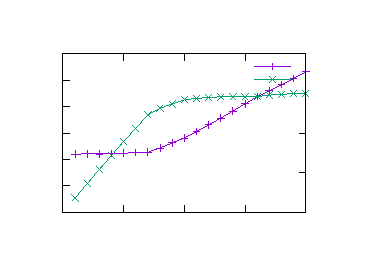
\includegraphics[width={170.00bp},height={113.30bp}]{out/tex/data/06axpb//cpu_latency_throughput_simd_m_big}}%
    \gplfronttext
  \end{picture}%
\endgroup
}
%out/tex/data/06axpy/simd\_m\_performance
\end{center}
\end{column}
\end{columns}

\begin{itemize}
\item the pattern is similar, but there are two differences:
  \begin{itemize}
  \item the \aka{latency} of a single update became $\approx$ \aka{11} cycles
  \item the \aka{throughput} hits the plateau at $\approx$ 24 flops/cycles
    ($\approx$ \aka{0.75} vfmaddps/cycle)
  \end{itemize}
\end{itemize}
\end{frame}

%%%%%%%%%%%%%%%%%%%%%%%%%%%%%%%%%% 
\begin{frame}[fragile]
\frametitle{Take a look at assembly}

\begin{itemize}
\item it looks like:
{\scriptsize
\begin{lstlisting}
.L1811:
  vmovaps %zmm0, %zmm2
  addq    $64, %rcx
  vfmadd132ps -64(%rcx), %zmm1, %zmm2
  vmovups %zmm2, -64(%rcx)
  cmpq    %rcx, %r8
  jne     .L1811
\end{lstlisting}} %$

\item what's the difference from the code 
  we have seen before (whose latency $=$ 4 cycles)?

{\scriptsize
\begin{lstlisting}
.L1800:
  addq    $1, %rdx
  vfmadd132ps %zmm0, %zmm1, %zmm2
  cmpq    %rdx, %rdi
  jne     .L1800
\end{lstlisting}} %$
\end{itemize}
\end{frame}

%%%%%%%%%%%%%%%%%%%%%%%%%%%%%%%%%% 
\begin{frame}
\frametitle{The reason of the \ao{\em latency} (11 cycles)}
\begin{itemize}
\item both stem from the fact that
  the code now involves load/stores

\item \ao{\it what you need to know:}
  \begin{quote}
  just like FMA, each instruction has its own latency  
  \end{quote}

\end{itemize}
\end{frame}

%%%%%%%%%%%%%%%%%%%%%%%%%%%%%%%%%% 
\begin{frame}
  \frametitle{Latencies of various instructions}

\begin{center}
{\small
  \begin{tabular}{|l|c|c|c|}\hline
instruction           & Haswell & Broadwell & Skylake \\\hline
  fp add              & 3       & 3         & \ao{4} \\
  fp mul              & 5       & 3         & \ao{4} \\
  fp fmadd            & 5       & 5         & \ao{4} \\
  typical integer ops & 1       & 1         & \ao{1} \\
  load                & 3       & 3         & \aka{3}($\ast$) \\
  store               & 4       & 4         & \aka{3}($\ast$) \\
  \ldots              & \ldots  & \ldots    & \ldots \\
\hline
  \end{tabular}
}
\end{center}


\begin{itemize}
\item $3 + 4 + 3 = 10 \neq 11$;
  I could not get information that confirms
  the extra cycle, but a simpler
  experiment shows the same result
  {\footnote (may be 512 bit store takes 4 cycles?)}
  
\begin{center}

\includegraphics[width=0.2\textwidth]{out/pdf/svg/i_got_it.pdf}  
\end{center}

\item I couldn't get the reliable source for it;
  Intel Intrinsics Guide says it is \aka{8 (!)} cycles, but
  I cannot believe it
\end{itemize}
\end{frame}

%%%%%%%%%%%%%%%%%%%%%%%%%%%%%%%%%% 
\begin{frame}
\frametitle{The reason of the \ao{\em throughput}}

\begin{itemize}
\item \ao{\emph{what you need to know:}}
  \begin{quote}
    Just like FMA, all instructions have their
    own throughput limits,
    due to 
    execution resources (dispatch ports and execution units)
\end{quote}

\item ``two \texttt{vfmadd}s per cycle'' is just an example of it

\end{itemize}

% \begin{columns}
% \begin{column}{0.6\textwidth}
% \begin{center}
% 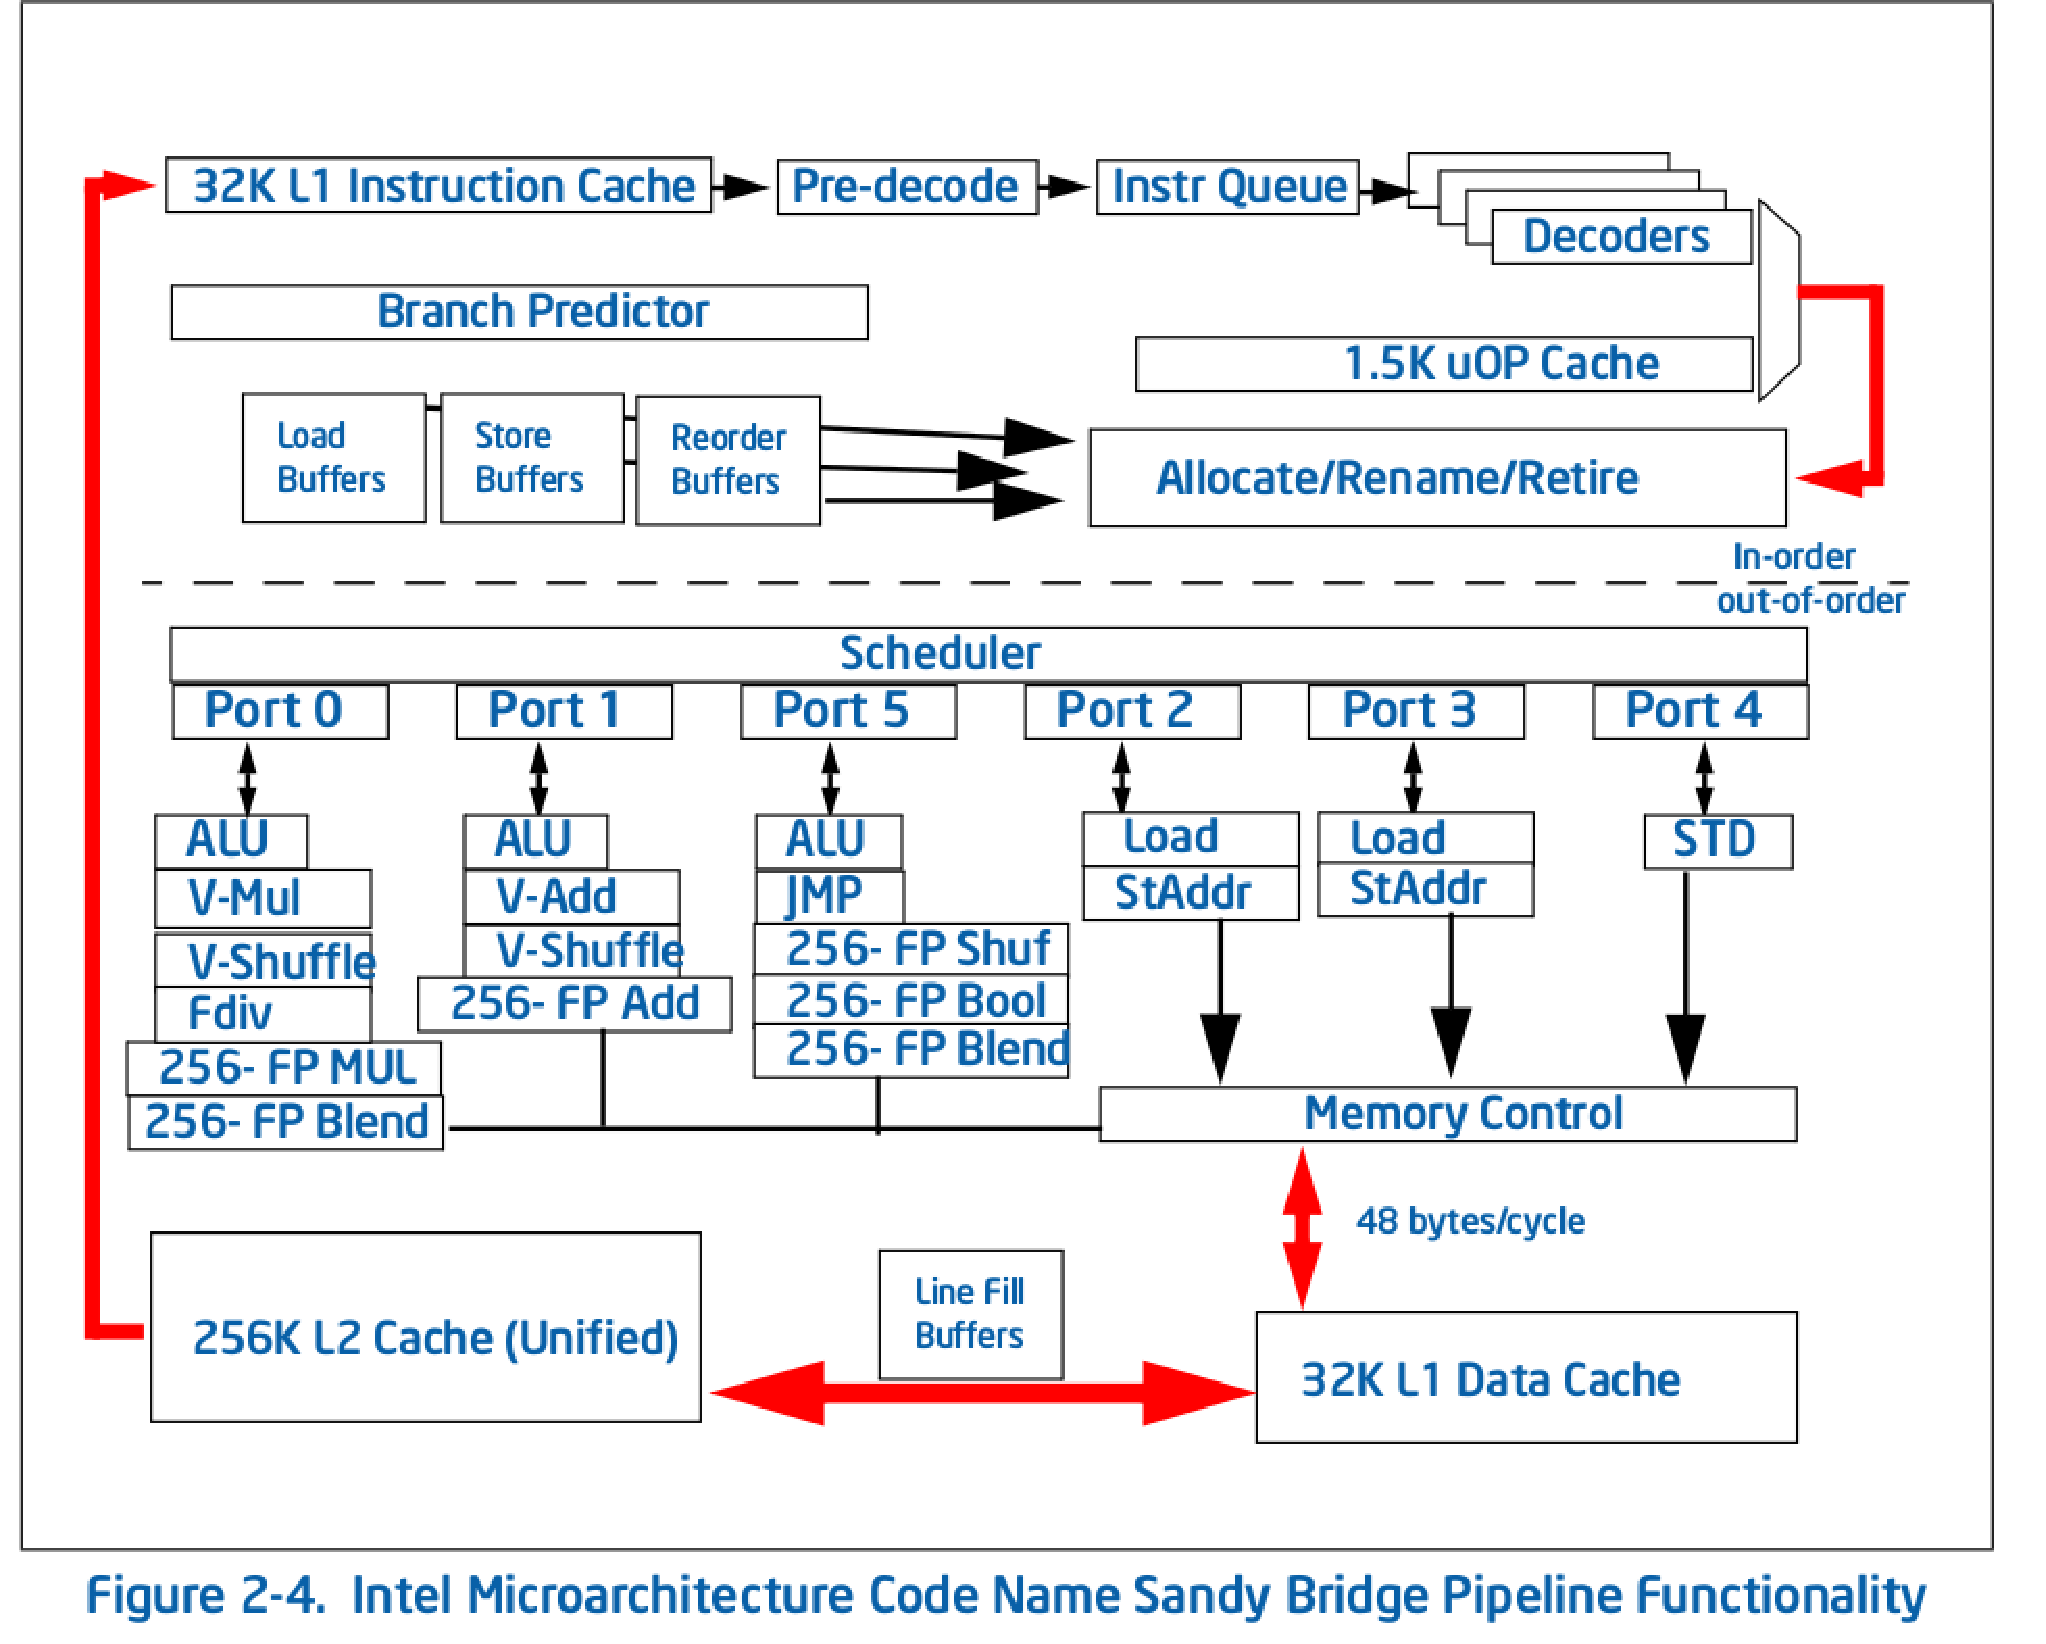
\includegraphics[width=0.8\textwidth]{out/pdf/img/sandybridge.pdf}

% {\tiny\em Intel 64 and IA-32 Architecture Optimization Reference Manual}
% \end{center}
% \end{column}
% \end{columns}
\end{frame}

%%%%%%%%%%%%%%%%%%%%%%%%%%%%%%%%%% 
\begin{frame}
\frametitle{Some representative throughput limits}

\begin{itemize}
\item Throughput $=$ the number of
  that instruction that can be executed by cycle

\begin{center}
{\small
  \begin{tabular}{|l|c|c|c|}\hline
instruction           & Haswell & Broadwell & Skylake \\\hline
  fp add/mul/fmadd    & 2       & 2         & 2 \\
  load                & 2       & 2         & 2 \\
  store               & 1       & 1         & \aka{1} \\
  typical integer ops & 4       & 4         & 4 \\
  \ldots              & \ldots  & \ldots    & \ldots \\
\hline
  \end{tabular}
}
\end{center}

\item Note: I couldn't get
  the reason for $\approx \aka{0.75} < 1$ (iterations/cycle)

\end{itemize}
\end{frame}

%%%%%%%%%%%%%%%%%%%%%%%%%%%%%%%%%%

\begin{frame}
\frametitle{A back of envelope calculation}

\begin{itemize}
\item []
{\scriptsize
  \begin{tabular}{|l|l|r|}\hline
    instruction & type & 1/throughput \\\hline
{\tt vmovaps \%zmm0,\%zmm2}  & register move & {\tiny 0.33} \\
{\tt addq \$64,\%rcx}     & int op & {\tiny 0.25} \\
{\tt vfmadd132ps -64(\%rcx),\%zmm1,\%zmm2} & load + FMA & 0.5, 0.5 \\
{\tt vmovups \%zmm2,-64(\%rcx)} & store & \aka{1.0} \\
{\tt cmpq \%rcx,\%r8} & compare & 0.25 \\
{\tt jne .L1811} & jump & 1-2 \\
\hline
  \end{tabular}}
\item I don't know what {\tt 1-2} means
\item we can conclude that the throughput $\leq 1$ due to the store

\item more general cases require understanding
  {\it dispatch ports}
\end{itemize}
\end{frame}


%%%%%%%%%%%%%%%%%%%%%%%%%%%%%%%%%% 
\begin{frame}[fragile]
\frametitle{Dispatch ports}
\begin{columns}
\begin{column}{0.5\textwidth}
\begin{itemize}
\item each instruction ($\mu$-operation) 
  is dispatched to a specific \ao{\emph{port}}
\item Skylake X ports
  \begin{itemize}
  \item fmadd $\rightarrow$ port 0 or 1
  \item load $\rightarrow$ port 2 or 3
  \item store $\rightarrow$ port 4
  \item load/store address generation $\rightarrow$ port 7
  \item int $\rightarrow$ port 0, 1, 5, or 6
  \item etc.
  \end{itemize}

\end{itemize}
\end{column}

\begin{column}{0.5\textwidth}
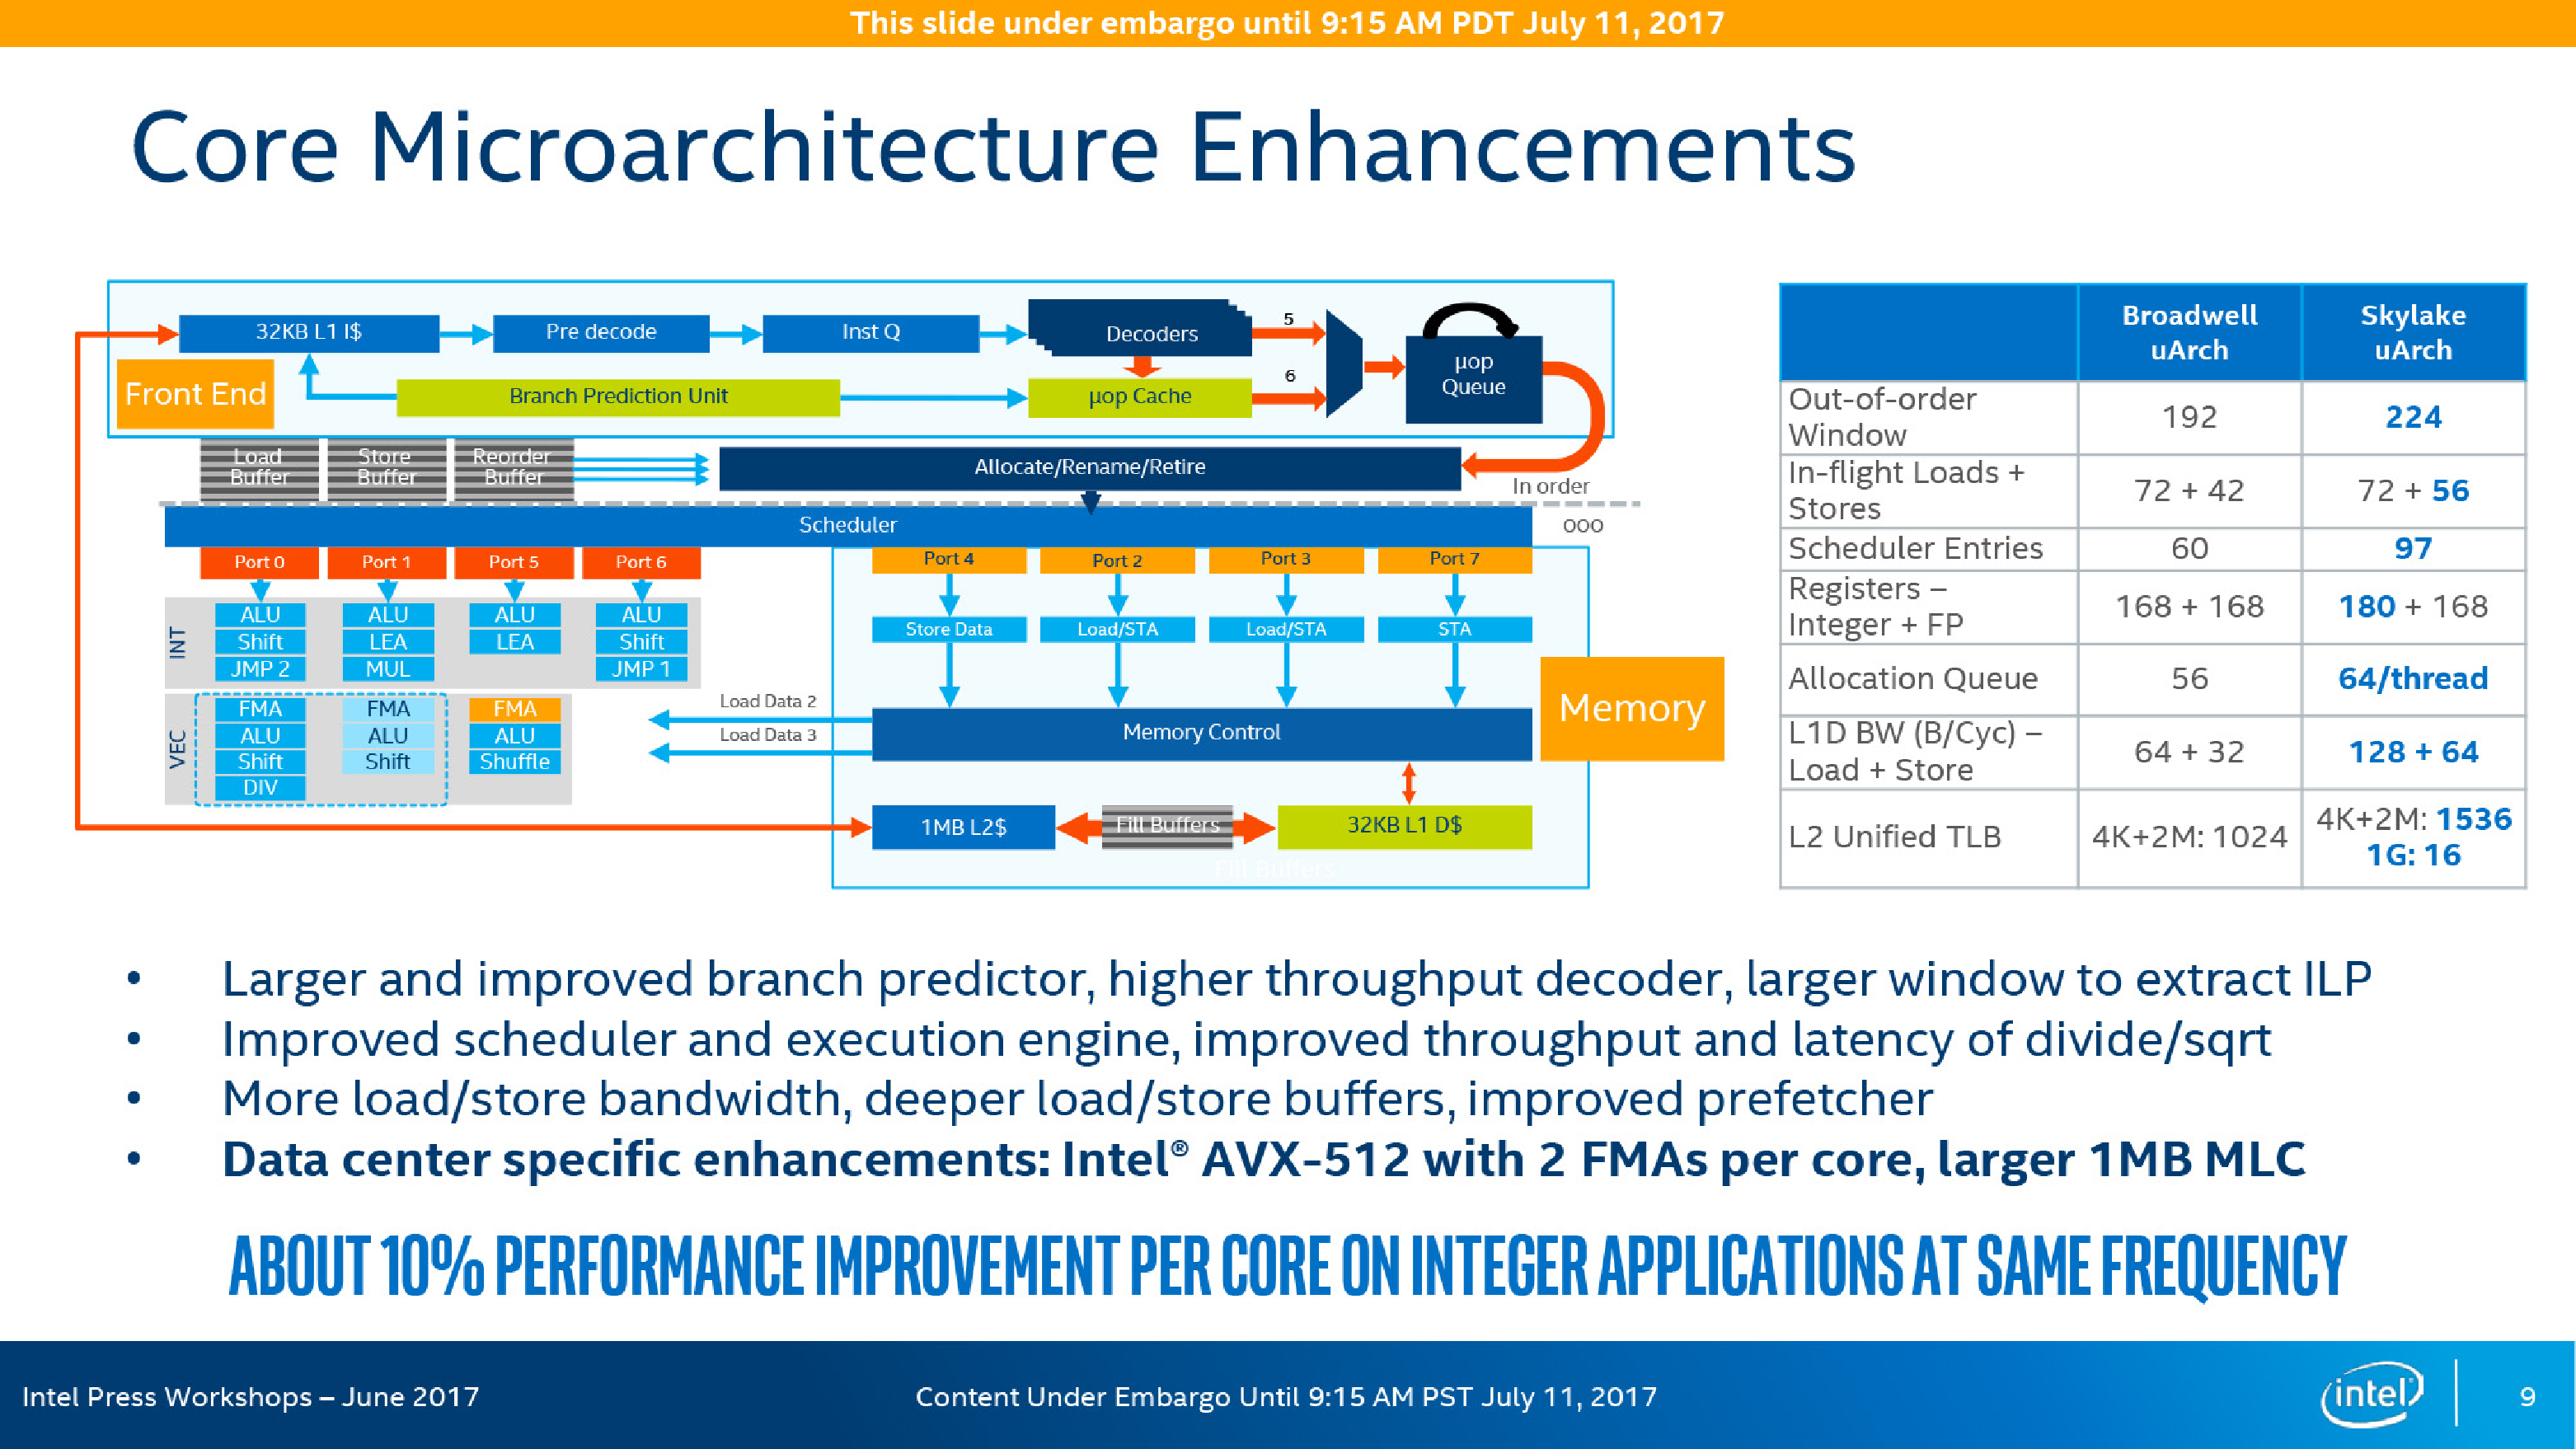
\includegraphics[width=\textwidth]{out/pdf/img/skylake_sp_buffer_windows.pdf}

{\tiny source: \url{https://en.wikichip.org/wiki/intel/microarchitectures/skylake_(server)}}
\end{column}
\end{columns}

\begin{itemize}
\item each port can take only a single operation per cycle
  \begin{itemize}
  \item this determines the aggregate throughput of all instructions
    that go to that port
  \end{itemize}
\item \ao{\it with destination ports of instructions, one can calculate
    the throughput limit of a given loop}
\end{itemize}
\end{frame}

%%%%%%%%%%%%%%%%%%%%%%%%%%%%%%%%%% 
\begin{frame}
\frametitle{Intel Architecture Code Analyzer}

\begin{itemize}
\item a great tool to analyze
  the throughput (and latency to some extent) limit
\item \url{https://software.intel.com/en-us/articles/intel-architecture-code-analyzer}

  \begin{center}
    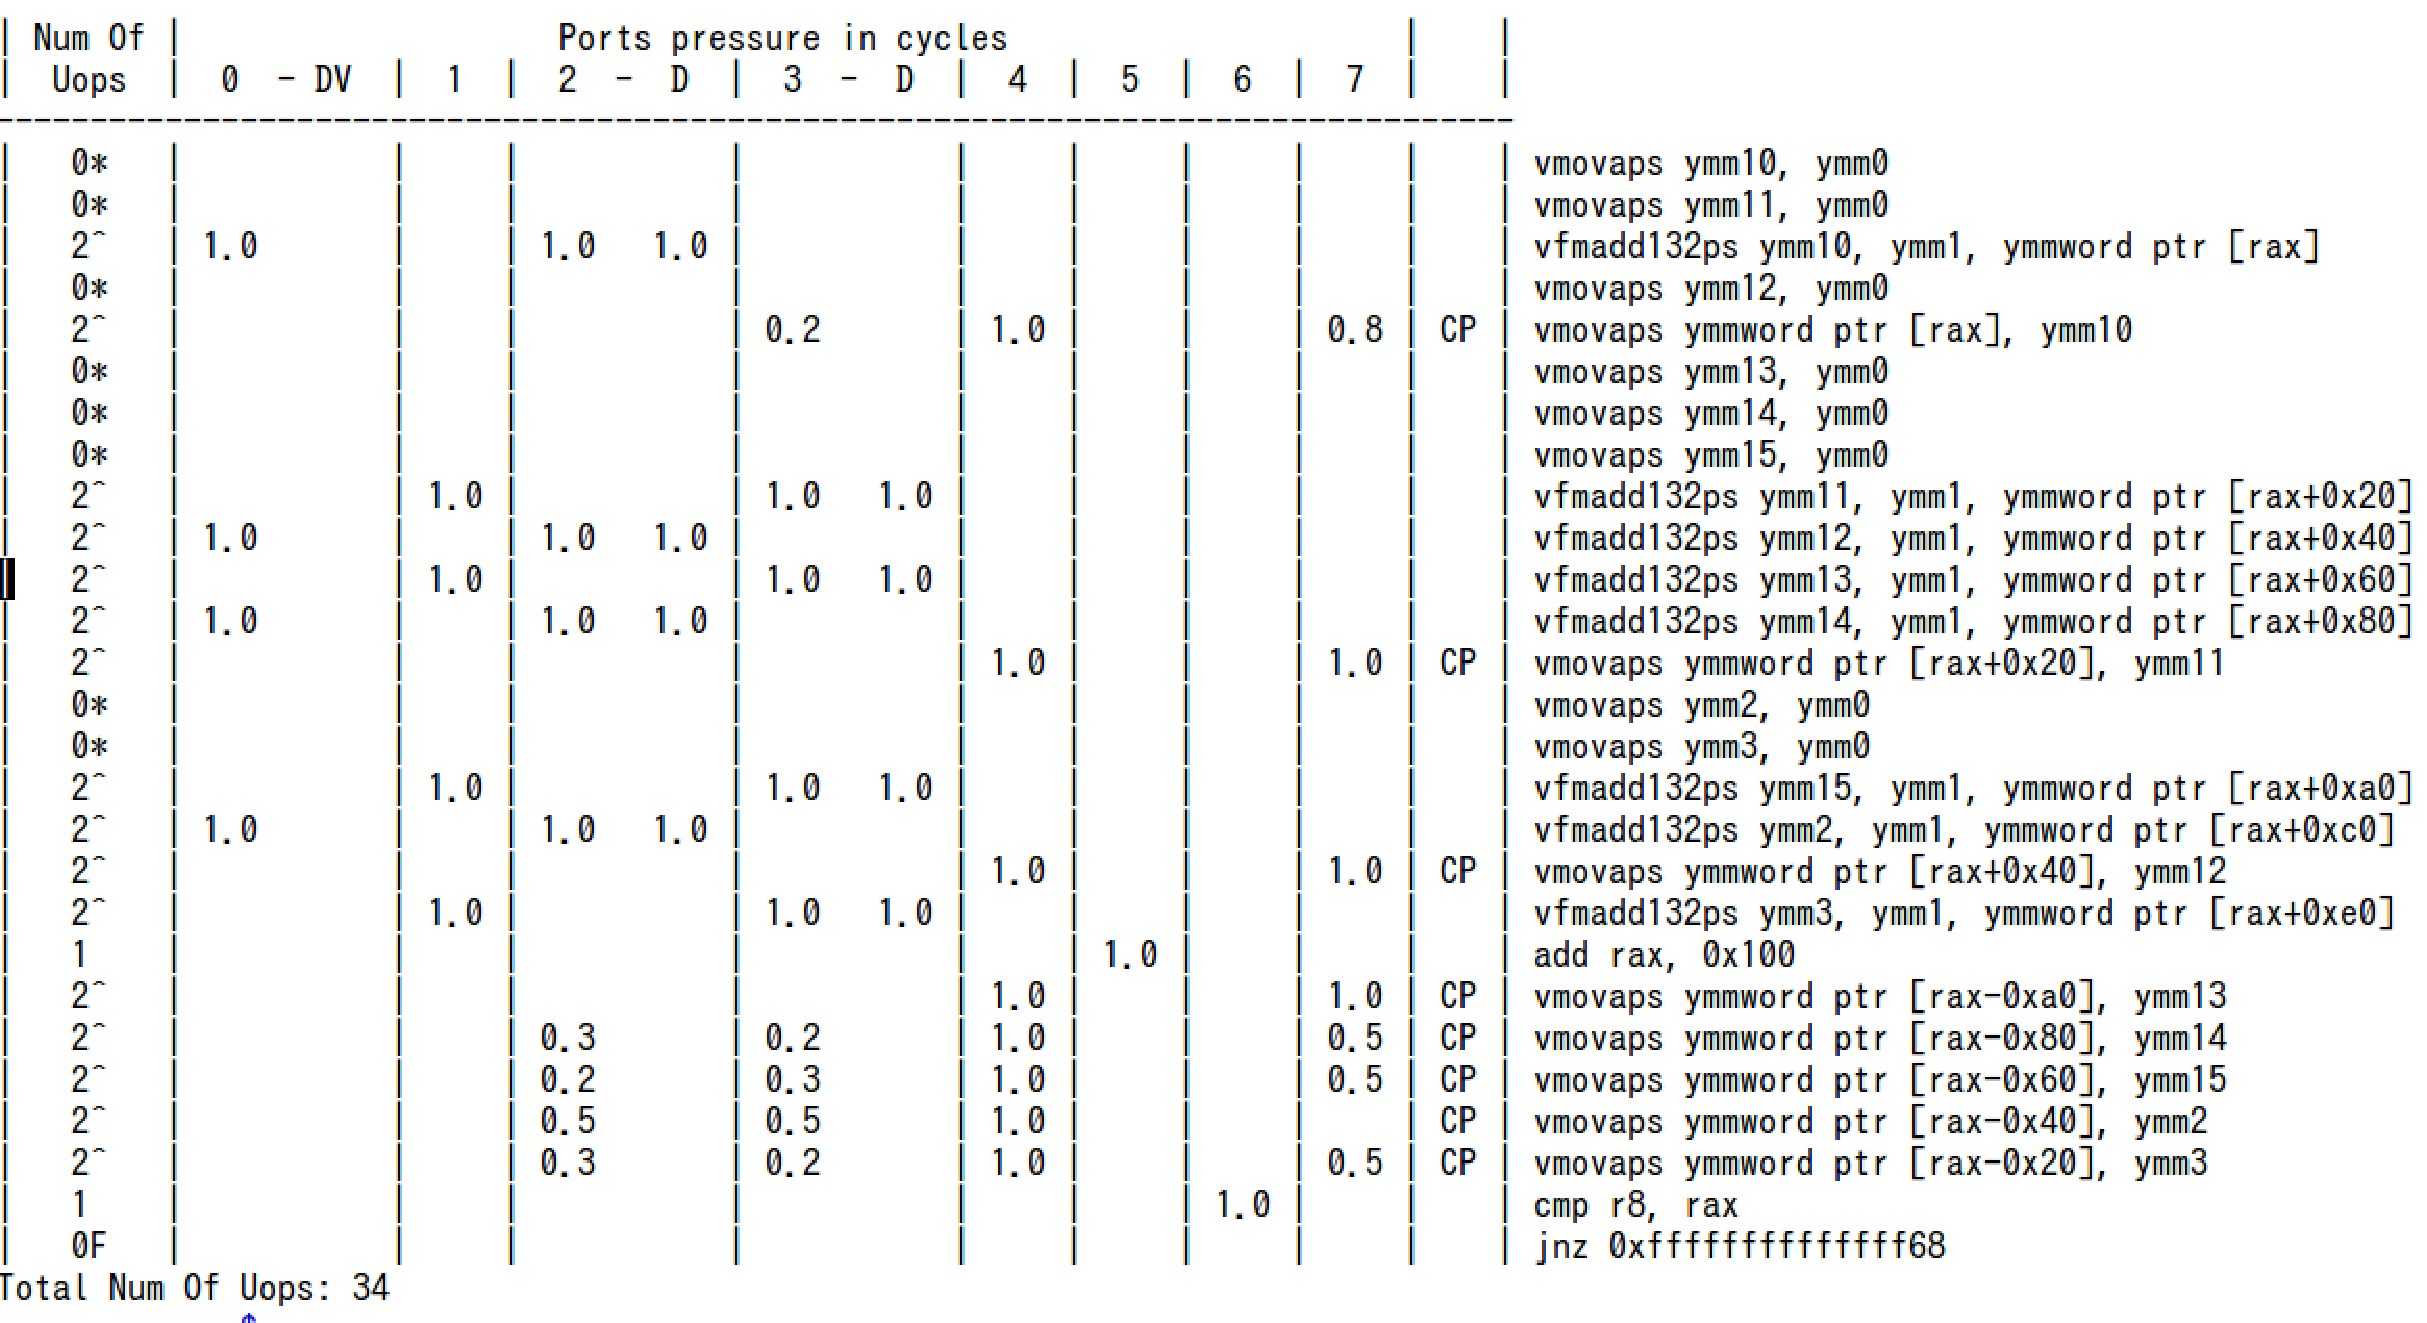
\includegraphics[width=0.8\textwidth]{out/pdf/img/iaca.pdf}
  \end{center}

\item checking the web site, I realized Intel now says it reached End Of Life and suggests use of LLVM-MCA (I will show it in the class)
\end{itemize}
\end{frame}

%%%%%%%%%%%%%%%%%%%%%%%%%%%%%%%%%% 
\begin{frame}[fragile]
\frametitle{How to overcome the throughput limit?}
\begin{itemize}
\item the goal is two iterations/cycle (throughput limit of FMA)
\item the bottleneck is a store instruction (1/cycle)
  
\item we obviously need to quit loading/storing
  data for every single fmadd
\begin{lstlisting}
for (i = 0; i < n; i++) {
  for (j = 0; j < nv; j++) {
    x[j] = a * x[j] + c; // load; fmadd; store
  }
}
\end{lstlisting}

\item the minimum ``unit'' of a computation
  should look like:

\begin{lstlisting}
load x[j] to a register;
@{\it do ``{\tt a * x + c}'' \ao{several times} on the register;}@
store the result to x[j];
\end{lstlisting}

\item and run multiple independent units
\end{itemize}
\end{frame}

%%%%%%%%%%%%%%%%%%%%%%%%%%%%%%%%%% 
\begin{frame}
\frametitle{Several ways to arrange computation}
\begin{columns}
\begin{column}{0.5\textwidth}
\begin{itemize}
\item {\small take a variable at a time and run it until the end (suffer from latency)}
\def\svgwidth{0.7\textwidth}
{\scriptsize \input{out/tex/svg/axpy2.pdf_tex}}
\item {\small advance all variables one step at a time (suffer from the store throughput)}
\def\svgwidth{0.7\textwidth}
{\scriptsize \input{out/tex/svg/axpy1.pdf_tex}}
\end{itemize}

\end{column}
\begin{column}{0.5\textwidth}
\begin{itemize}
\item {\small strategy 1: take a few variables and run them until the end}
\def\svgwidth{0.7\textwidth}
{\scriptsize \input{out/tex/svg/axpy3.pdf_tex}}
\item {\small strategy 2: advance all variables, a few steps at a time}
\def\svgwidth{0.7\textwidth}
{\scriptsize \input{out/tex/svg/axpy4.pdf_tex}}
\end{itemize}
\end{column}
\end{columns}
\end{frame}

%%%%%%%%%%%%%%%%%%%%%%%%%%%%%%%%%% 
\begin{frame}[fragile]
\frametitle{Implementing strategy 1}
\begin{itemize}
\item say we advance ten elements at a time
\begin{lstlisting}
for (j = 0; j < nv; j += b) {
  @\mura{\it/* run b variables until the end */}@
  for (i = 0; i < n; i++) {
    for (jj = j; jj < j + b; jj++) {
      @\mura{\tt xx[jj] =}@ a * @\mura{\tt xx[jj]}@ + c;
    }
  }
}
\end{lstlisting}

\item we hope it loads/stores each
  variable only once through the $i$ loop (line 2)!
\item this coding \ao{\em depends on the compiler's smartness} we have witnessed
  \begin{itemize}
  \item promote fixed-sized arrays into registers
  \end{itemize}
\end{itemize}
\end{frame}

%%%%%%%%%%%%%%%%%%%%%%%%%%%%%%%%%% 
\begin{frame}[fragile]
\frametitle{Implementing strategy 2}
\begin{itemize}
\item advance all variables, say three, steps at a time
\begin{lstlisting}
for (i = 0; i < n; i += 3) {
  @\mura{\it/* run all variables 3 steps */}@
  for (j = 0; j < m; j++) {
    for (ii = 0; ii < 3; ii++) {
      @\mura{\tt x[j] =}@ a * @\mura{\tt x[j]}@ + c;
    }
  }
}
\end{lstlisting}

\item again, we hope the compiler's smartness
  to eliminate intermediate load/stores (\mura{purple
    parts})

\item the latency of a single $j$ iteration
  increases, but we hope the $j$ loop exposes
  lots of independent computations
\end{itemize}
\end{frame}

%%%%%%%%%%%%%%%%%%%%%%%%%%%%%%%%%% 
\begin{frame}
\frametitle{Results (strategy I)}

\begin{columns}[t]
\begin{column}{0.35\textwidth}
  \begin{center}
    \vskip0.5cm
{\scriptsize
\begin{tabular}{|c|c|c|}\hline
chains & clocks/iter & flops/clock \\
\hline
1 & 4.002 & 7.994 \\
2 & 4.001 & 15.992 \\
3 & 4.005 & 23.968 \\
4 & 4.014 & 31.886 \\
5 & 4.021 & 39.788 \\
6 & 4.022 & 47.734 \\
7 & 4.133 & 54.196 \\
8 & 4.032 & 63.478 \\
9 & 4.599 & 62.613 \\
10 & 5.034 & 63.558 \\
11 & 5.539 & 63.544 \\
12 & 6.051 & 63.452 \\
13 & 6.538 & 63.628 \\
14 & 7.043 & 63.608 \\
15 & 7.544 & 63.626 \\
16 & 8.044 & 63.646 \\
\hline
\end{tabular}}
\end{center}
\end{column}

\begin{column}{0.65\textwidth}
\begin{center}
%{\scriptsize \input{out/tex/data/06axpy/simd_m_mnm_performance}}
%out/tex/data/06axpy/simd\_m\_mnm\_performance
  {\tiny % GNUPLOT: LaTeX picture with Postscript
\begingroup
  \makeatletter
  \providecommand\color[2][]{%
    \GenericError{(gnuplot) \space\space\space\@spaces}{%
      Package color not loaded in conjunction with
      terminal option `colourtext'%
    }{See the gnuplot documentation for explanation.%
    }{Either use 'blacktext' in gnuplot or load the package
      color.sty in LaTeX.}%
    \renewcommand\color[2][]{}%
  }%
  \providecommand\includegraphics[2][]{%
    \GenericError{(gnuplot) \space\space\space\@spaces}{%
      Package graphicx or graphics not loaded%
    }{See the gnuplot documentation for explanation.%
    }{The gnuplot epslatex terminal needs graphicx.sty or graphics.sty.}%
    \renewcommand\includegraphics[2][]{}%
  }%
  \providecommand\rotatebox[2]{#2}%
  \@ifundefined{ifGPcolor}{%
    \newif\ifGPcolor
    \GPcolortrue
  }{}%
  \@ifundefined{ifGPblacktext}{%
    \newif\ifGPblacktext
    \GPblacktexttrue
  }{}%
  % define a \g@addto@macro without @ in the name:
  \let\gplgaddtomacro\g@addto@macro
  % define empty templates for all commands taking text:
  \gdef\gplbacktext{}%
  \gdef\gplfronttext{}%
  \makeatother
  \ifGPblacktext
    % no textcolor at all
    \def\colorrgb#1{}%
    \def\colorgray#1{}%
  \else
    % gray or color?
    \ifGPcolor
      \def\colorrgb#1{\color[rgb]{#1}}%
      \def\colorgray#1{\color[gray]{#1}}%
      \expandafter\def\csname LTw\endcsname{\color{white}}%
      \expandafter\def\csname LTb\endcsname{\color{black}}%
      \expandafter\def\csname LTa\endcsname{\color{black}}%
      \expandafter\def\csname LT0\endcsname{\color[rgb]{1,0,0}}%
      \expandafter\def\csname LT1\endcsname{\color[rgb]{0,1,0}}%
      \expandafter\def\csname LT2\endcsname{\color[rgb]{0,0,1}}%
      \expandafter\def\csname LT3\endcsname{\color[rgb]{1,0,1}}%
      \expandafter\def\csname LT4\endcsname{\color[rgb]{0,1,1}}%
      \expandafter\def\csname LT5\endcsname{\color[rgb]{1,1,0}}%
      \expandafter\def\csname LT6\endcsname{\color[rgb]{0,0,0}}%
      \expandafter\def\csname LT7\endcsname{\color[rgb]{1,0.3,0}}%
      \expandafter\def\csname LT8\endcsname{\color[rgb]{0.5,0.5,0.5}}%
    \else
      % gray
      \def\colorrgb#1{\color{black}}%
      \def\colorgray#1{\color[gray]{#1}}%
      \expandafter\def\csname LTw\endcsname{\color{white}}%
      \expandafter\def\csname LTb\endcsname{\color{black}}%
      \expandafter\def\csname LTa\endcsname{\color{black}}%
      \expandafter\def\csname LT0\endcsname{\color{black}}%
      \expandafter\def\csname LT1\endcsname{\color{black}}%
      \expandafter\def\csname LT2\endcsname{\color{black}}%
      \expandafter\def\csname LT3\endcsname{\color{black}}%
      \expandafter\def\csname LT4\endcsname{\color{black}}%
      \expandafter\def\csname LT5\endcsname{\color{black}}%
      \expandafter\def\csname LT6\endcsname{\color{black}}%
      \expandafter\def\csname LT7\endcsname{\color{black}}%
      \expandafter\def\csname LT8\endcsname{\color{black}}%
    \fi
  \fi
    \setlength{\unitlength}{0.0500bp}%
    \ifx\gptboxheight\undefined%
      \newlength{\gptboxheight}%
      \newlength{\gptboxwidth}%
      \newsavebox{\gptboxtext}%
    \fi%
    \setlength{\fboxrule}{0.5pt}%
    \setlength{\fboxsep}{1pt}%
    \definecolor{tbcol}{rgb}{1,1,1}%
\begin{picture}(3400.00,2266.00)%
    \gplgaddtomacro\gplbacktext{%
      \csname LTb\endcsname%%
      \put(300,384){\makebox(0,0)[r]{\strut{}$0$}}%
      \put(300,553){\makebox(0,0)[r]{\strut{}$1$}}%
      \put(300,722){\makebox(0,0)[r]{\strut{}$2$}}%
      \put(300,891){\makebox(0,0)[r]{\strut{}$3$}}%
      \put(300,1060){\makebox(0,0)[r]{\strut{}$4$}}%
      \put(300,1229){\makebox(0,0)[r]{\strut{}$5$}}%
      \put(300,1398){\makebox(0,0)[r]{\strut{}$6$}}%
      \put(300,1567){\makebox(0,0)[r]{\strut{}$7$}}%
      \put(300,1736){\makebox(0,0)[r]{\strut{}$8$}}%
      \put(300,1905){\makebox(0,0)[r]{\strut{}$9$}}%
      \put(372,264){\makebox(0,0){\strut{}$0$}}%
      \put(672,264){\makebox(0,0){\strut{}$2$}}%
      \put(973,264){\makebox(0,0){\strut{}$4$}}%
      \put(1273,264){\makebox(0,0){\strut{}$6$}}%
      \put(1574,264){\makebox(0,0){\strut{}$8$}}%
      \put(1874,264){\makebox(0,0){\strut{}$10$}}%
      \put(2174,264){\makebox(0,0){\strut{}$12$}}%
      \put(2475,264){\makebox(0,0){\strut{}$14$}}%
      \put(2775,264){\makebox(0,0){\strut{}$16$}}%
      \put(2847,384){\makebox(0,0)[l]{\strut{}$0$}}%
      \put(2847,574){\makebox(0,0)[l]{\strut{}$8$}}%
      \put(2847,764){\makebox(0,0)[l]{\strut{}$16$}}%
      \put(2847,954){\makebox(0,0)[l]{\strut{}$24$}}%
      \put(2847,1145){\makebox(0,0)[l]{\strut{}$32$}}%
      \put(2847,1335){\makebox(0,0)[l]{\strut{}$40$}}%
      \put(2847,1525){\makebox(0,0)[l]{\strut{}$48$}}%
      \put(2847,1715){\makebox(0,0)[l]{\strut{}$56$}}%
      \put(2847,1905){\makebox(0,0)[l]{\strut{}$64$}}%
    }%
    \gplgaddtomacro\gplfronttext{%
      \csname LTb\endcsname%%
      \put(2208,1782){\makebox(0,0)[r]{\strut{}latency}}%
      \csname LTb\endcsname%%
      \put(2208,1662){\makebox(0,0)[r]{\strut{}throughput}}%
      \csname LTb\endcsname%%
      \put(114,1144){\rotatebox{-270.00}{\makebox(0,0){\strut{}cycles/iter}}}%
      \put(3123,1144){\rotatebox{-270.00}{\makebox(0,0){\strut{}flops/cycle}}}%
      \put(1573,84){\makebox(0,0){\strut{}inner variables}}%
      \put(1573,2085){\makebox(0,0){\strut{}a compile-time constant number of variables in the innermost loop}}%
    }%
    \gplbacktext
    \put(0,0){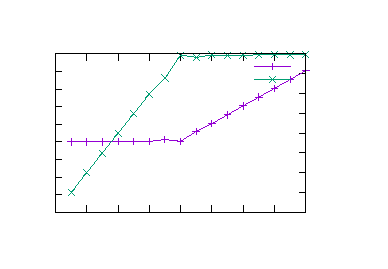
\includegraphics[width={170.00bp},height={113.30bp}]{out/tex/data/06axpb//cpu_latency_throughput_simd_m_mnm_big}}%
    \gplfronttext
  \end{picture}%
\endgroup
}
\end{center}
\end{column}
\end{columns}

\end{frame}

\iffalse
%%%%%%%%%%%%%%%%%%%%%%%%%%%%%%%%%% 
\begin{frame}
\frametitle{Results}
\begin{itemize}
\item strategy 1: succeeded 
  \begin{itemize}
  \item $\approx$ 31.92 flops/clock out of 32 flops/clock; 99.75\% of the peak
  \end{itemize}
\item strategy 2: 
  not as successful as strategy 1 
  \begin{itemize}
  \item $\approx$ 27.82 flops/clock; (87\% of the peak)
  \end{itemize}

% \item why?
% \end{itemize}

% \begin{center}
% {\scriptsize \input{out/tex/gpl/chain_3steps_flops}}
% \end{center}
\end{itemize}
\end{frame}
%%%%%%%%%%%%%%%%%%%%%%%%%%%%%%%%%% 
\begin{frame}
\frametitle{Reason of suboptimal results for strategy 2}
\begin{itemize}
\item<1-> again, latency is the issue, but in a subtler way

\item<2-> the processor decodes instructions in the order issued by the program
  \ao{\emph{(program order)}}

\item<3-> it can execute instructions ($\mu$-operations) 
  whose operands arrive \ao{\emph{(out of order execution)}}

\item<4-> $\Rightarrow$ operations whose operands are not ready are put 
  in a buffer \ao{\emph{reservation station}}
\end{itemize}

\begin{center}
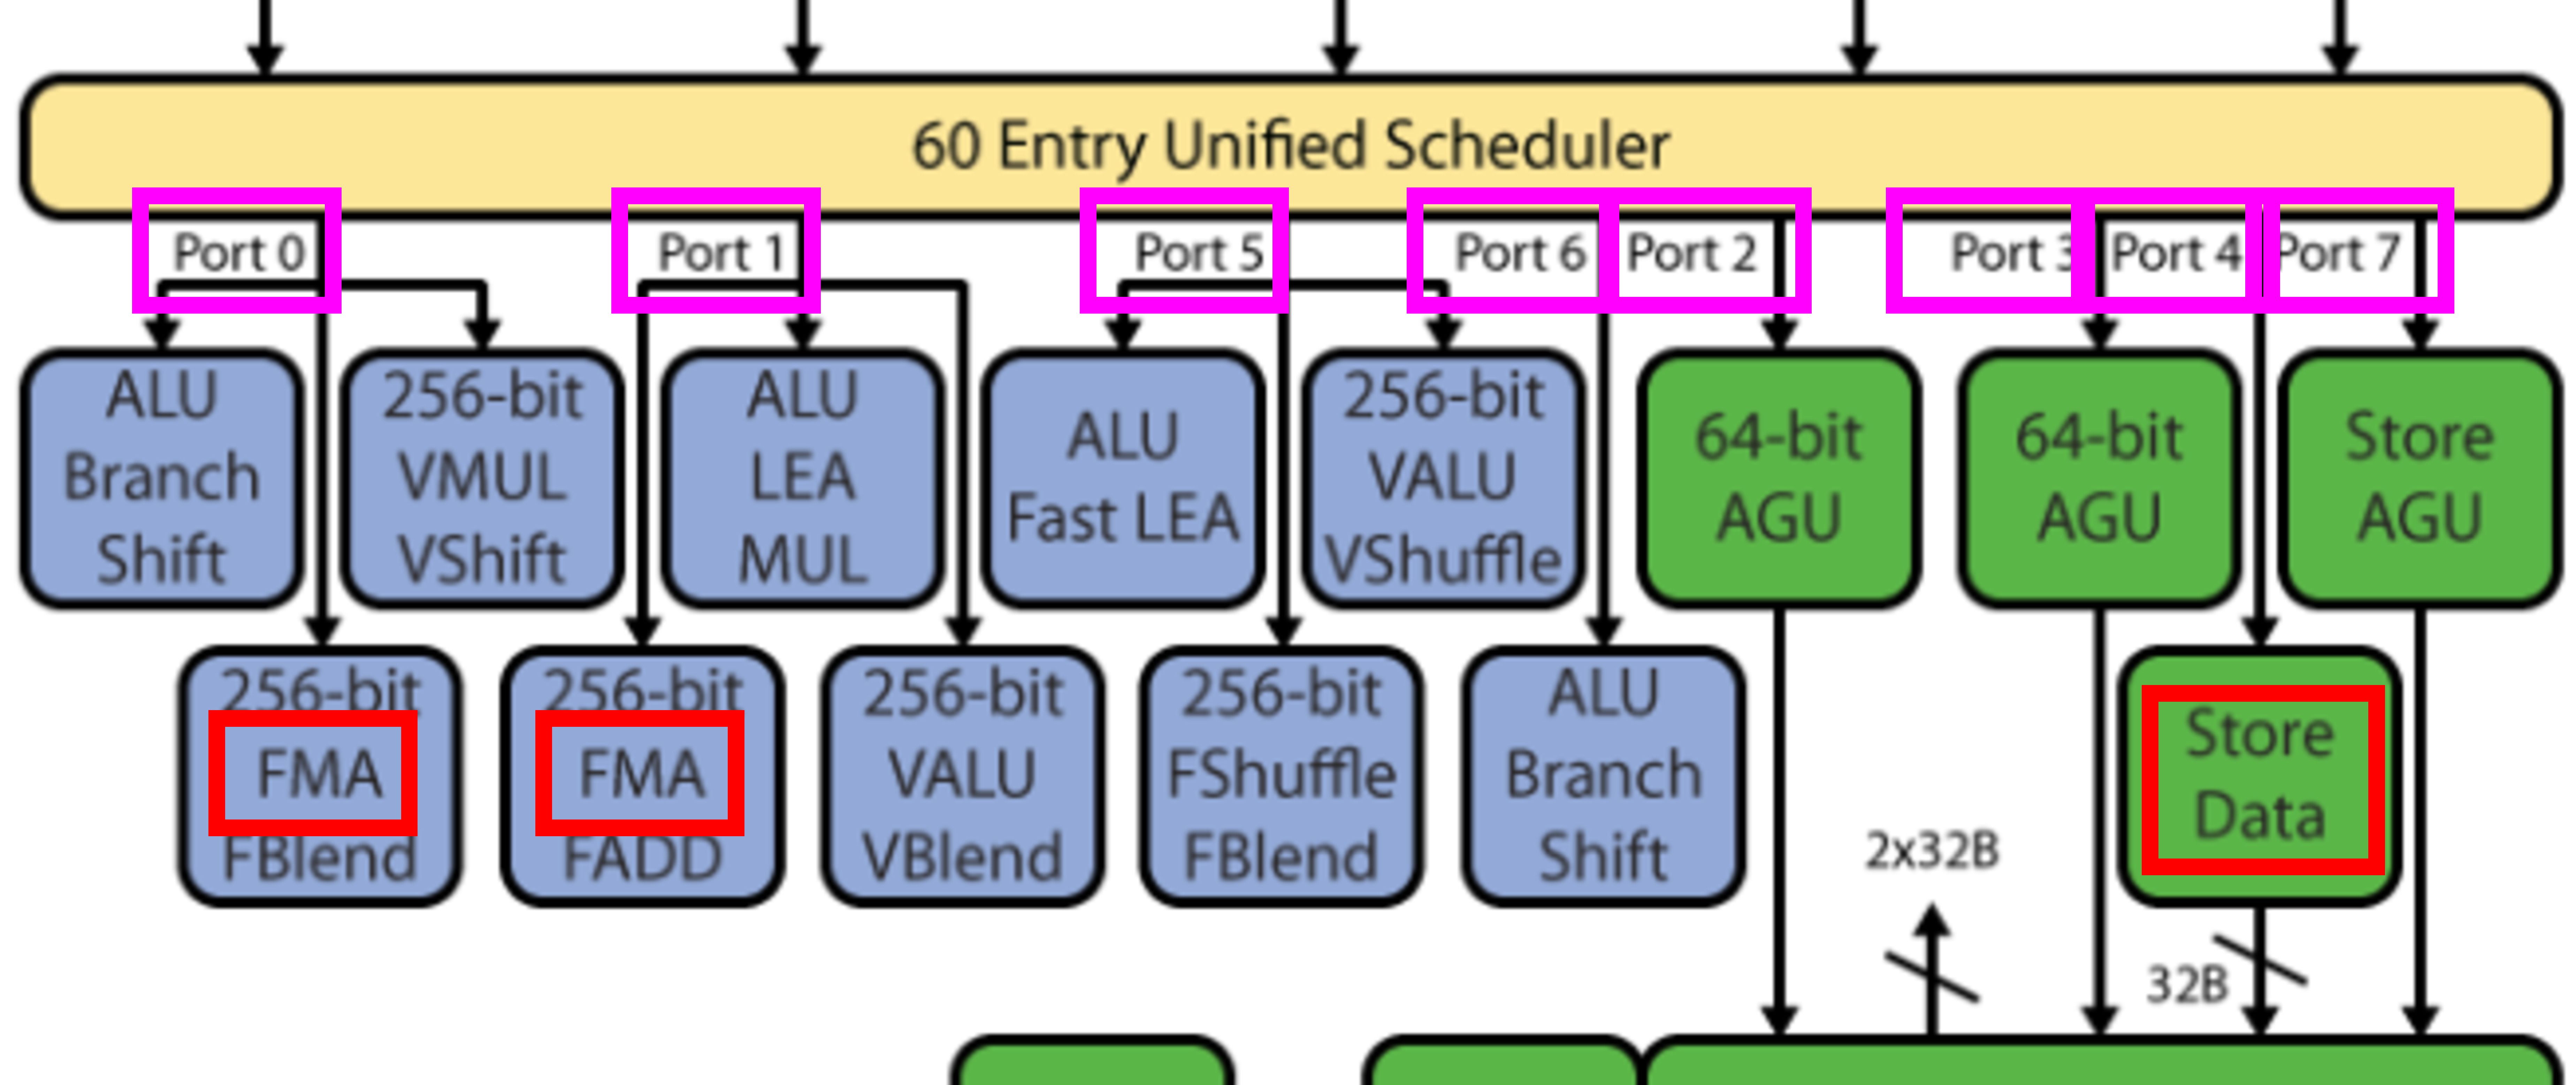
\includegraphics[width=0.5\textwidth]{out/pdf/svg/haswell_ports.pdf}
%\def\svgwidth{0.5\textwidth}
%{\scriptsize \input{out/tex/svg/out_of_order_broadwell_1.pdf_tex}}%
\end{center}
\end{frame}

%%%%%%%%%%%%%%%%%%%%%%%%%%%%%%%%%% 
\begin{frame}
\frametitle{Reason of suboptimal results for strategy 2}
\begin{itemize}
\item<1-> but the reservation station (any physical resource in a processor, for that matter) 
  is finite (Haswell has 60 entries) % sandy bridge 54
\item<2-> $\Rightarrow$ the processor can keep only so many operations waiting 
\item<3-> when the reservation station is full, the processor
  \aka{\em cannot decode} any more instructions 
  (even if some of the following instructions can be immediately executed)
\end{itemize}
\end{frame}

%%%%%%%%%%%%%%%%%%%%%%%%%%%%%%%%%% 
\begin{frame}
\frametitle{Implication of finite reservation station}
\begin{itemize}
\item instructions must enter the reservation station
  in the program order
\item instructions near the tail of a long dependency chain
  occupies entries for a long time
\begin{center}
\def\svgwidth{0.7\textwidth}
{\scriptsize \input{out/tex/svg/broadwell_reservation.pdf_tex}}
\end{center}

\item if there are too many such instructions,
  the processor cannot decode instructions 
  further ahead and fail to find otherwise executable
  instructions
\end{itemize}
\end{frame}
\fi


\fi

%%%%%%%%%%%%%%%%%%%%%%%%%%%%%%%%%% 
%%%%%%%%%%%%%%%%%%%%%%%%%%%%%%%%%% 
\section{A simple yet fairly fast single-core matrix multiply}
%%%%%%%%%%%%%%%%%%%%%%%%%%%%%%%%%% 
%%%%%%%%%%%%%%%%%%%%%%%%%%%%%%%%%%

%%%%%%%%%%%%%%%%%%%%%%%%%%%%%%%%%% 
\begin{frame}
\frametitle{Developing near peak FLOPS matrix multiply}
\begin{itemize}
\item let's develop a (single core) matrix multiply that runs
  at fairly good FLOPS on Ice Lake
\item it is a great application of the concept you have just learned
\[ C = A * B + C \]
\item []
\begin{center}

\only<1>{\def\svgwidth{0.5\textwidth}{\scriptsize \input{out/tex/svg/mm_1.pdf_tex}}}%
\only<2>{\def\svgwidth{0.4\textwidth}{\scriptsize \input{out/tex/svg/mm_2.pdf_tex}}}
\end{center}

\end{itemize}
\end{frame}

%%%%%%%%%%%%%%%%%%%%%%%%%%%%%%%%%% 
\begin{frame}
\frametitle{A few convenient assumptions}
\begin{itemize}
\item we add assumptions that $M$, $N$, and $K$ 
  are multiple of certain numbers along the way,
  (don't worry about ``remainder'' rows/columns)

\item we assume matrix sizes are conveniently small (don't worry about
  memory access cost, which is actually a significant factor to design
  matrix multiply for larger matrices)

\item multiplication of larger (and unknown size) matrices can be
  built on top of this
\end{itemize}
\end{frame}

%%%%%%%%%%%%%%%%%%%%%%%%%%%%%%%%%% 
\begin{frame}[fragile]
\frametitle{Step 1: Baseline code}

\begin{columns}
  \begin{column}{0.55\textwidth}
\begin{center}
\def\svgwidth{0.8\textwidth}
{\scriptsize \input{out/tex/svg/mm_3.pdf_tex}}
\end{center}
  \end{column}
  \begin{column}{0.4\textwidth}
\begin{lstlisting}
$ mm_base 8 32 192
M = 8, N = 32, K = 192
L : 16
A : 8 x 192 (ld=192) 6144 bytes
B : 192 x 32 (ld=32) 24576 bytes
C : 8 x 32 (ld=32) 1024 bytes
total = 31744 bytes
repeat : 20346 times
perform 1000046592 fmas ... done
2844287815 clocks
0.351598 fmas/cycle
\end{lstlisting}%$
  \end{column}
\end{columns}

\begin{itemize}
\item []
\begin{lstlisting}
for (i = 0; i < M; i++)  
  for (j = 0; j < N; j++)  
    for (k = 0; k < K; k++)  
      C(i,j) += A(i,k) * B(k,j);
\end{lstlisting}
\end{itemize}

\begin{itemize}
\item it runs at $\approx$ 2.8 clocks / innermost loop
\end{itemize}
\end{frame}

%%%%%%%%%%%%%%%%%%%%%%%%%%%%%%%%%% 
\begin{frame}[fragile]
\frametitle{Step 1: analysis}
\begin{itemize}
\item latency limit : latency of FMA
  \begin{itemize}
  \item the reason why it's slightly {\it smaller} than 4
    is there are some overlaps between different elements of $C$
  \item if you set $M = N = 1$ and $K$ large, it's almost exactly 4
  \end{itemize}
\item throughput limit : not important

\item achieved performance :
  1000046592 fmas / 2844287815 cycles $\approx$ \ao{0.4} fmas/cycle
\end{itemize}
\end{frame}

%%%%%%%%%%%%%%%%%%%%%%%%%%%%%%%%%% 
\begin{frame}[fragile]
\frametitle{Step 2: Vectorization}
\begin{columns}
  \begin{column}{0.55\textwidth}
\begin{center}
\def\svgwidth{0.8\textwidth}
\only<1>{\scriptsize \input{out/tex/svg/mm_3.pdf_tex}}%
\only<2->{\scriptsize \input{out/tex/svg/mm_4.pdf_tex}}%
\end{center}
  \end{column}
  \begin{column}{0.4\textwidth}
\begin{lstlisting}
$ mm_simd 8 32 192
M = 8, N = 32, K = 192
L : 16
A : 8 x 192 (ld=192) 6144 bytes
B : 192 x 32 (ld=32) 24576 bytes
C : 8 x 32 (ld=32) 1024 bytes
total = 31744 bytes
repeat : 20346 times
perform 1000046592 fmas ... done
180175475 clocks
5.550404 fmas/cycle
\end{lstlisting}%$
  \end{column}
\end{columns}

\begin{itemize}
\item []
\begin{lstlisting}
for (i = 0; i < M; i++)  
  for (j = 0; j < N; j += L)
    for (k = 0; k < K; k++)  
      @\ao{\texttt{C(i,j:j+L) += A(i,k) * B(k,j:j+L);}}@
\end{lstlisting}
\end{itemize}

\begin{itemize}
\item assumption: $N$ is a multiple of SIMD lanes ($L$)
\item it still runs at $\approx$ 2.8 clocks / innermost iteration
\end{itemize}
\end{frame}

%%%%%%%%%%%%%%%%%%%%%%%%%%%%%%%%%% 
\begin{frame}[fragile]
\frametitle{Step 2: analysis}
\begin{itemize}
  
\item the speed is still limited by latency
\item the only difference is that each iteration now performs 16 fmas (as opposed to an fma)

\item achieved throughput :

  \[ 1000046592 \mbox{ fmas} / 180175475 \mbox{ cycles} \approx 5.5 \mbox{ fmas/cycle} \]
\end{itemize}
\end{frame}

%%%%%%%%%%%%%%%%%%%%%%%%%%%%%%%%%% 
\begin{frame}[fragile]
\frametitle{Step 3: increase parallelism!}
\begin{columns}
  \begin{column}{0.55\textwidth}
\begin{center}
\def\svgwidth{0.8\textwidth}
\only<1>{\scriptsize \input{out/tex/svg/mm_4.pdf_tex}}%
\only<2->{\scriptsize \input{out/tex/svg/mm_5.pdf_tex}}%
\end{center}
  \end{column}
  \begin{column}{0.4\textwidth}
\begin{lstlisting}
$ ./mm_simd_ilp 8 32 192
M = 8, N = 32, K = 192
L : 16
A : 8 x 192 (ld=192) 6144 bytes
B : 192 x 32 (ld=32) 24576 bytes
C : 8 x 32 (ld=32) 1024 bytes
total = 31744 bytes
repeat : 20346 times
perform 1000046592 fmas ... done
64836630 clocks
15.424099 fmas/cycle
\end{lstlisting}%$
  \end{column}
\end{columns}

\begin{itemize}
\item update {\it bM} vector elements of $C$ concurrently
\begin{lstlisting}
for (i = 0; i < M; i += bM)
  for (j = 0; j < N; j += L)  
    for (k = 0; k < K; k++)  
      @\ao{\texttt{for (di = 0; di < bM; di++)}}@
        @\ao{\texttt{C(i+di,j:j+L) += A(i+di,k) * B(k,j:j+L);}}@
\end{lstlisting}

\item Ice Lake requires {\it bM} $\geq 8$ to reach peak FLOPS
\end{itemize}
\end{frame}

%%%%%%%%%%%%%%%%%%%%%%%%%%%%%%%%%% 
\begin{frame}[fragile]
  \frametitle{Step 3: analysis}
  \begin{columns}
    \begin{column}{0.35\textwidth}
\begin{center}
\def\svgwidth{0.9\textwidth}
{\scriptsize \input{out/tex/svg/mm_5.pdf_tex}}%
\end{center}
    \end{column}
    \begin{column}{0.58\textwidth}
\begin{lstlisting}
for (i = 0; i < M; i += bM)
 for (j = 0; j < N; j += L)  
  for (k = 0; k < K; k++)  
   @\ao{\texttt{for (di = 0; di < bM; di++)}}@
    @\ao{\texttt{C(i+di,j:j+L) += A(i+di,k) * B(k,j:j+L);}}@
\end{lstlisting}
    \end{column}
  \end{columns}

\begin{itemize}
\item the for loop at line 4 performs
  \begin{itemize}
  \item \ao{\it bM} loads (broadcasts) for {\tt A(i+di,k)}
  \item \ao{\it 1} load for {\tt B(k,j:j+L)}
  \item \ao{\it bM} FMAs
  \end{itemize}
\item the load/broadcast throughput $=$ 2 per cycle
\item to achieve 2 FMAs/cycle, we must have
  \[ \mbox{the number of broadcast} \leq \mbox{the number of FMAs} \]
\end{itemize}
\end{frame}

%%%%%%%%%%%%%%%%%%%%%%%%%%%%%%%%%% 
\begin{frame}[fragile]
\frametitle{Step 4: Reuse an element of $A$}
\begin{columns}
  \begin{column}{0.55\textwidth}
\begin{center}
\def\svgwidth{0.8\textwidth}
{\scriptsize \input{out/tex/svg/mm_6.pdf_tex}}%
\end{center}
  \end{column}
  \begin{column}{0.4\textwidth}
    \begin{lstlisting}
$ mm_simd_lip_4x2 8 32 192
M = 8, N = 32, K = 192
L : 16
A : 8 x 192 (ld=192) 6144 bytes
B : 192 x 32 (ld=32) 24576 bytes
C : 8 x 32 (ld=32) 1024 bytes
total = 31744 bytes
repeat : 20346 times
perform 1000046592 fmas ... done
38635137 clocks
25.884381 fmas/cycle
    \end{lstlisting} %$
  \end{column}
\end{columns}
\begin{itemize}
\item update {\it bM'} $\times$ {\it bN} block rather than
  {\it bM} $\times$ 1 
\begin{lstlisting}
for (i = 0; i < M; i += bM')  
  for (j = 0; j < N; j += bN * L)  
    for (k = 0; k < K; k++)  
      @\ao{\texttt{for (di = 0; di < bM'; di++)  }}@
        @\ao{\texttt{for (dj = 0; dj < bN * L; dj += L)}}@
          @\ao{\texttt{C(i+di,j+dj:j+dj+L) += A(i+di,k) * B(k,j+dj:j+L);}}@
\end{lstlisting}
\end{itemize}
\end{frame}


%%%%%%%%%%%%%%%%%%%%%%%%%%%%%%%%%% 
\begin{frame}
\frametitle{Step 4: Analysis}
\begin{itemize}
\item the for loop at line 4 performs
  \begin{itemize}
  \item \ao{\it bM'} loads (broadcast) for {\tt A(i+di,k)}
  \item \ao{\it bN} loads for {\tt B(k,j:j+L)}
  \item \ao{\it bM'} $\times$ \ao{\it bN} SIMD FMAs
  \end{itemize}
  
\item the minimum requirement for it to achieve the peak FLOPS is
  \ao{\it bM'} $\times$ \ao{\it bN} $\geq$ 8
\item in the experiments, when we set {\it bM'} $= 8$ and {\it bN} $= 2$, it gets
  \ao{25} fmas/cycle ($\approx$ \ao{80\%} of the peak)
\item we need to note that this happens only when the matrix is small
  ($M = 8, N = 32, K = 192$) and we repeat it many times
\item the issue for large matrices will be the next topic
\end{itemize}

\end{frame}

\iffalse
%%%%%%%%%%%%%%%%%%%%%%%%%%%%%%%%%% 
\begin{frame}
  \frametitle{Simultaneous Multithreading (SMT)}
\begin{itemize}
\item each physical core has several
  \ao{\it hardware threads} or \ao{\it virtual cores}
  \begin{itemize}
  \item recent Xeon processors (including Skylake-X) : 2
  \item Knights Landing/Mill : 4
  \item IBM Power : 8
  \end{itemize}
\item a.k.a. Hyperthreading$^{\mbox{\textregistered}}$
\item virtual cores on a single physical core
  \begin{itemize}
  \item are concurrently executed by the hardware
  \item have their own registers (switching between them have almost no overhead)
  \item \ao{\it share most execution resources}
    (dispatch ports, floating point units, L1/L2 caches, etc.)
  \end{itemize}
\end{itemize}
\begin{center}
  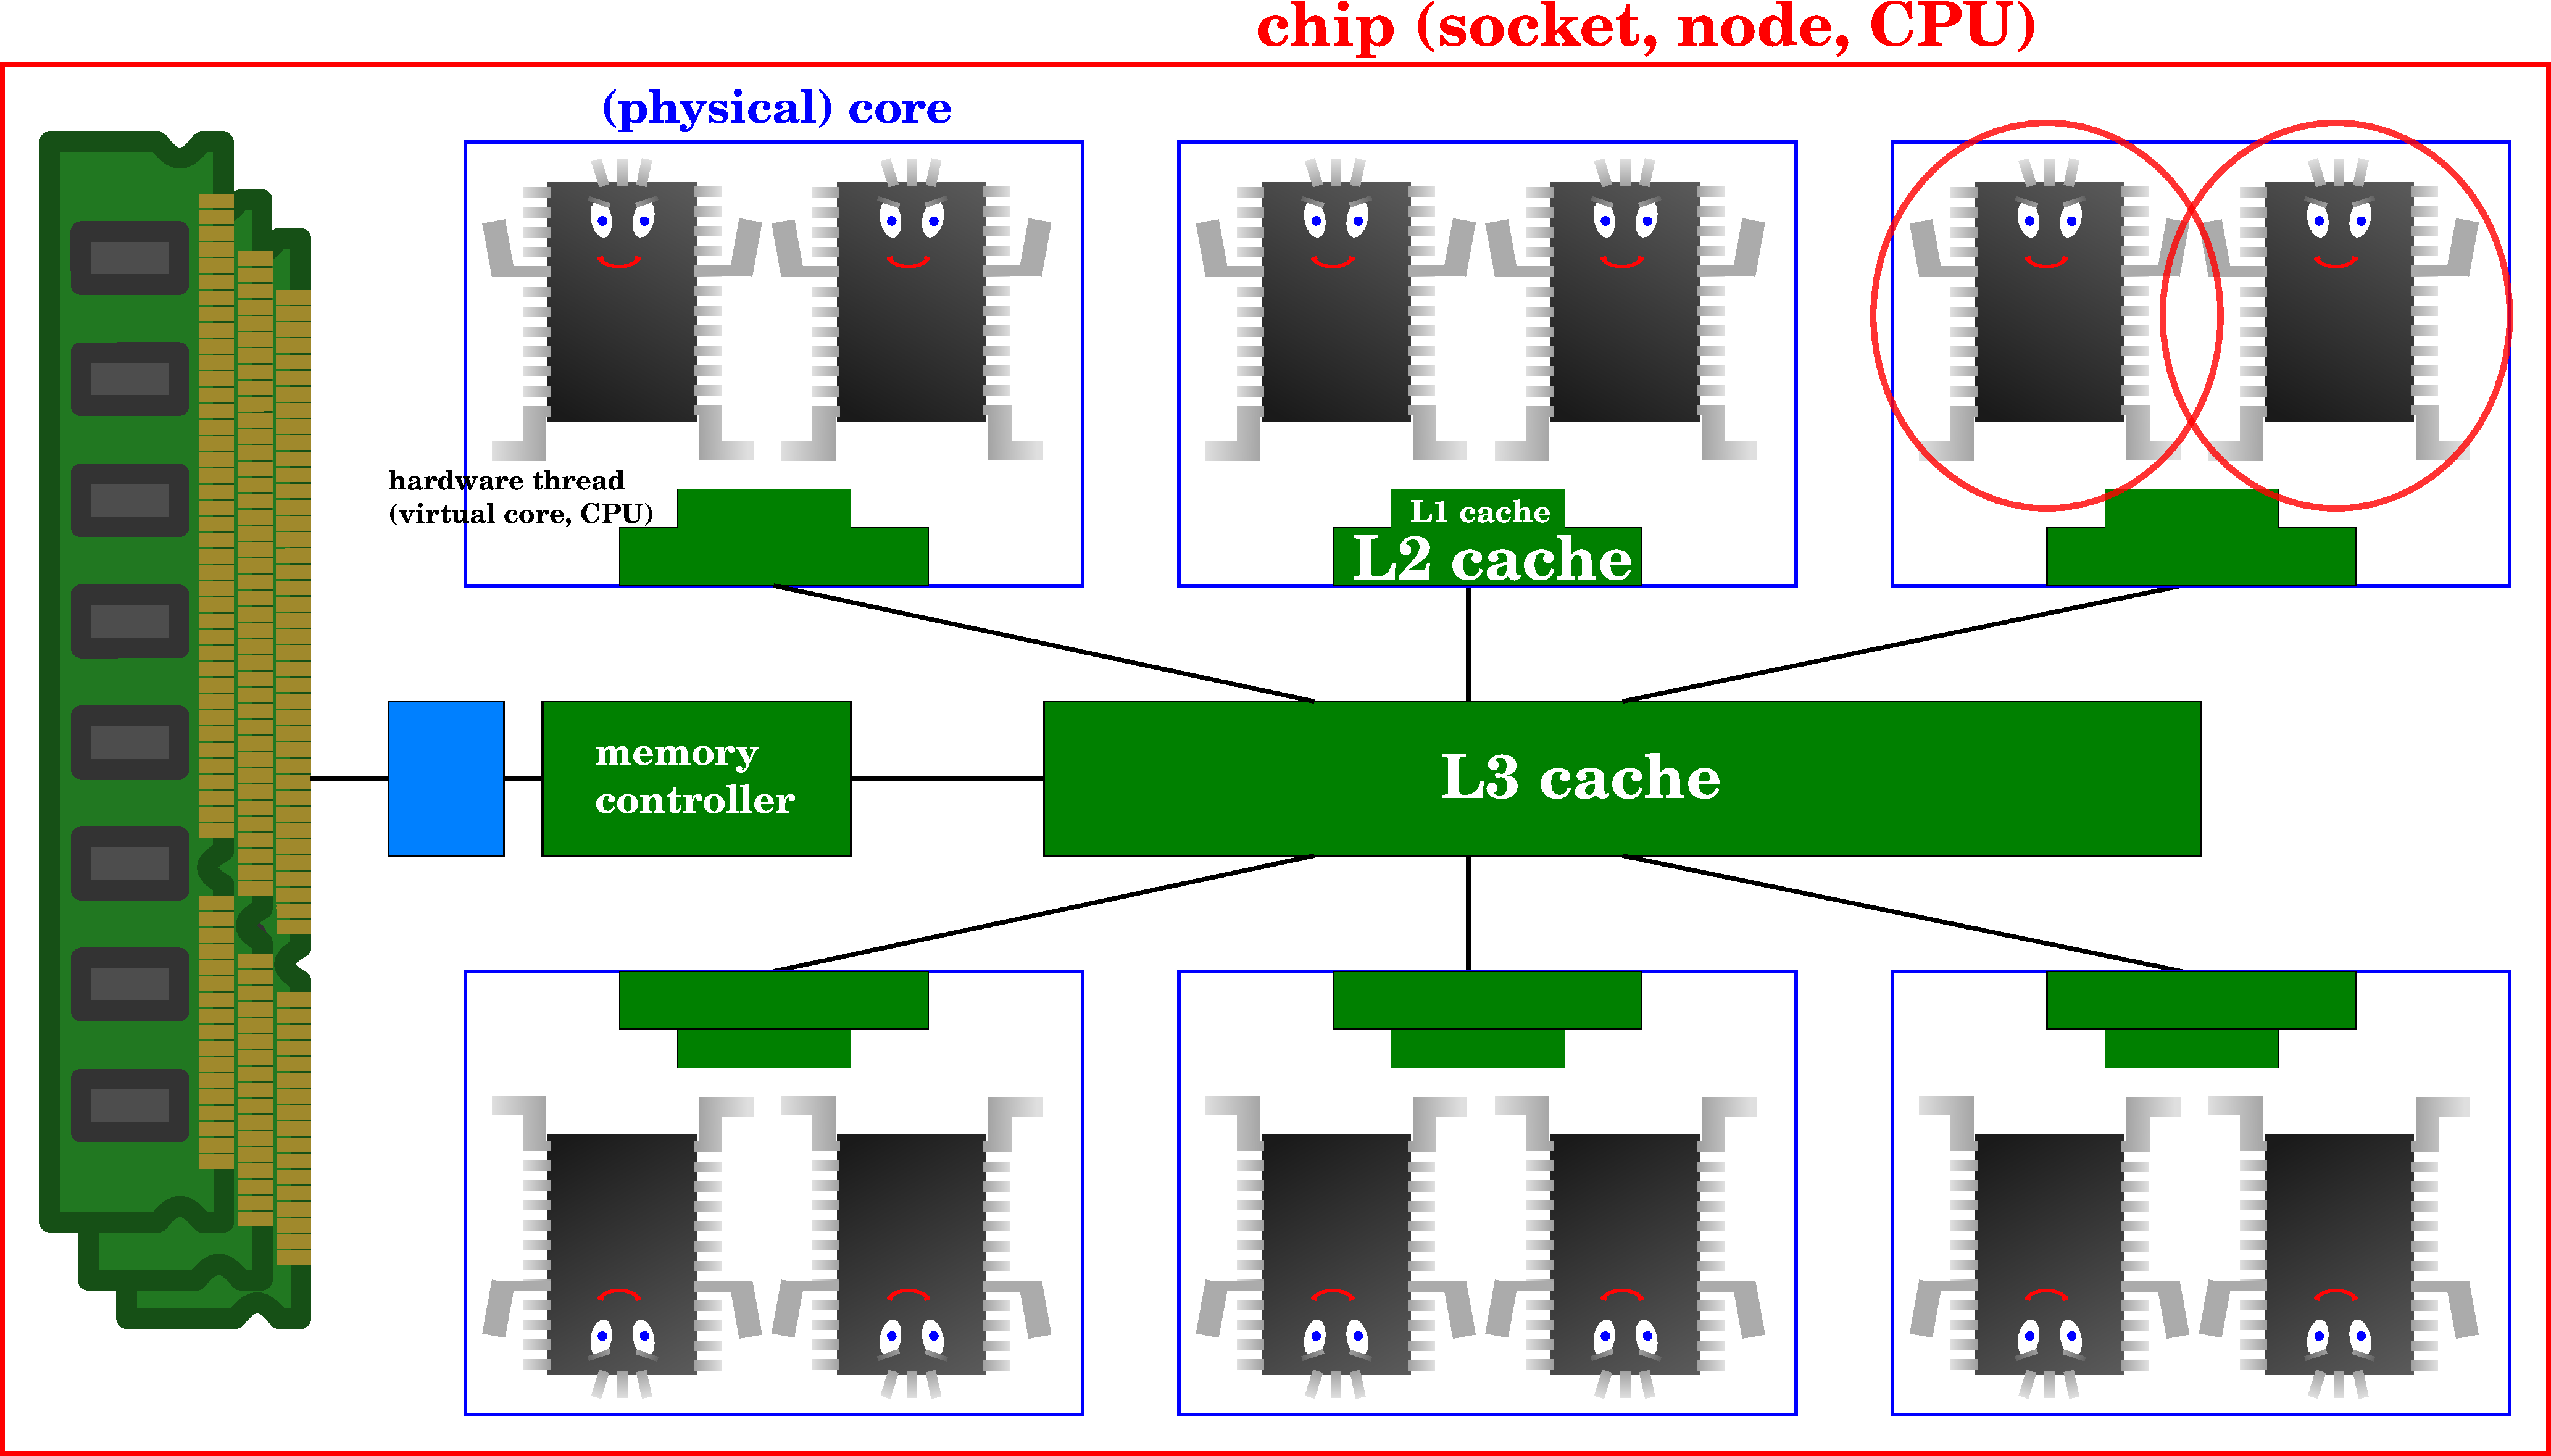
\includegraphics[width=0.3\textwidth]{out/pdf/svg/diagram_smt.pdf}
\end{center}

\end{frame}

%%%%%%%%%%%%%%%%%%%%%%%%%%%%%%%%%% 
\begin{frame}
\frametitle{Performance implications of virtual cores}
\begin{itemize}
\item having as many threads as virtual cores on a physical core
  \begin{itemize}
  \item helps improve throughput of \ao{\it latency-bound} applications, but 
  \item does not help \ao{\it throughput-bound} applications
  \end{itemize}

\item note: if you have more threads than virtual cores, operating systems get involved
  to switch between them (in a much coarser granularity, say 1 ms ($10^{-3}$ sec)
  rather than every cycle $\sim$ 1 ns ($10^{-9}$ sec))
  \begin{itemize}
  \item it never helps mitigate the latency of arithmetic operations
  \item it helps mitigate the latency of much bigger I/O latencies
    (say when accessing HDD)
  \end{itemize}
\end{itemize}
\end{frame}
\fi

%%%%%%%%%%%%%%%%%%%%%%%%%%%%%%%%%% 
\begin{frame}
\frametitle{Takeaways (1)}
\begin{itemize}
\item peak FLOPS of many recent Intel CPUs
  $=$ ``execute two \texttt{fmadd}s every cycle'' \aka{\it (no other combinations)}
  \begin{itemize}
  \item other processors have different limits, but the basics is the same
  \item cf. NVIDIA GPUs $=$ ``execute two warps (each doing \texttt{fmadd}) every cycle''
  \end{itemize}
\item single-core performance is not about reducing the number of instructions
\item it's about how to increase parallelism
  \begin{itemize}
  \item CPU : SIMD $\times$ ILP
  \item GPU : threads, threads, threads, \ldots 
  \item but the internal machinery is similar (warp $\approx$ SIMD, ILP $\sim$ warps in an SM)
  \item how they expose parallelism to the programmer is different
  \end{itemize}
\end{itemize}
\end{frame}

%%%%%%%%%%%%%%%%%%%%%%%%%%%%%%%%%% 
\begin{frame}
\frametitle{Takeaways (2)}
\begin{itemize}
\item dependent instructions incur latencies and hinder parallelism
\begin{center}
\def\svgwidth{0.6\textwidth}
{\scriptsize \input{out/tex/svg/long_chain1.pdf_tex}}
\end{center}

\item independent instructions are executed in parallel, 
  up to throughput limits
\begin{center}
\def\svgwidth{0.6\textwidth}
{\scriptsize \input{out/tex/svg/long_chain2.pdf_tex}}
\end{center}

\item throughput limits are determined by dispatch ports
\end{itemize}
\end{frame}



\end{document}

% \iffalse
% \item waiting instructions occupy a reservation station entry, 
%   so you'd better avoid issuing deeply dependent instructions too early
% \begin{center}
% \def\svgwidth{0.6\textwidth}
% {\scriptsize \input{out/tex/svg/long_chain3.pdf_tex}}
% \end{center}
% \fi


\iffalse
%%%%%%%%%%%%%%%%%%%%%%%%%%%%%%%%%% 
\begin{frame}
\frametitle{Takeaways (3)}
\begin{itemize}
\item the processor cannot execute 
  ``a serial chain of dependency'' that fast (throughput $=$ 1/latency)
\begin{center}
\def\svgwidth{0.6\textwidth}
{\scriptsize \input{out/tex/svg/long_chain1.pdf_tex}}
\end{center}

\item have a number of independent chains and gain throughput
\begin{center}
\def\svgwidth{0.6\textwidth}
{\scriptsize \input{out/tex/svg/long_chain2.pdf_tex}}
\end{center}

\item avoid putting long-waiting instructions upstream
\begin{center}
\def\svgwidth{0.6\textwidth}
{\scriptsize \input{out/tex/svg/long_chain3.pdf_tex}}
\end{center}

\item peak FLOPS is rarely achievable, but trying
to achieve it is a great learning opportunity
(of superscalar processors)

\end{itemize}
\end{frame}
\fi

%%%%%%%%%%%%%%%%%%%%%%%%%%%%%%%%%% 
\begin{frame}
\frametitle{Summary : what is CPU performance?}
\begin{itemize}
\item []
  \begin{quote}
CPU performance $=$ ILP $\times$ SIMD $\times$ multicores
\end{quote}

\item none is negligible

\item in an ideal world, the compiler does them all, but 
  you often times need to use them by yourself
  
\end{itemize}
\end{frame}

\end{document}


